%----------------------------------------------------------------------------------------
%	PACKAGES AND THEMES
%----------------------------------------------------------------------------------------
\PassOptionsToPackage{table}{xcolor}
\documentclass[aspectratio=169,xcolor=dvipsnames,svgnames,x11names,fleqn]{beamer}
% \documentclass[aspectratio=169,xcolor=dvipsnames,fleqn]{beamer}

\usetheme{RedVelvet}

\usefonttheme[onlymath]{serif}



\usepackage{xspace}
\usepackage{amsmath}
\usepackage{amssymb}
\usepackage{amsfonts}
\usepackage{color}
\usepackage{physics}
% \usepackage{mathbb}
\usepackage{rahul_math}
\usepackage{bigints}

\usepackage{graphicx} % Allows including images
\usepackage{booktabs} % Allows the use of \toprule, \midrule and \bottomrule in tables
\usepackage{tikz,pgfplots}

\usepackage{subfigure}
\usetikzlibrary{arrows}
\usepackage{minted}
\definecolor{LightGray}{gray}{0.9}
\definecolor{cream}{rgb}{0.92, 0.9, 0.55}
\definecolor{lightblue}{rgb}{0.68, 0.85, 0.9}


\usepackage{xcolor-material}
\usetikzlibrary{fit}
\usetikzlibrary{matrix}
\tikzset{%
apple/.pic={
  \fill [MaterialBrown] (-1/8,0)  arc (180:120:1 and 3/2) coordinate [pos=3/5] (@)-- ++(1/6,-1/7)  arc (120:180:5/4 and 3/2) -- cycle;
  \fill [MaterialLightGreen500] (0,-9/10)  .. controls ++(180:1/8) and ++(  0:1/4) .. (-1/3,  -1) .. controls ++(180:1/3) and ++(270:1/2) .. (  -1,   0) .. controls ++( 90:1/3) and ++(180:1/3) .. (-1/2, 3/4) .. controls ++(  0:1/8) and ++(135:1/8) .. (   0, 4/7)
}
}

\newcommand{\leftdoublequote}{\textcolor{blue}{\scalebox{3}{``}}}

\newcommand{\rightdoublequote}{\textcolor{blue}{\scalebox{3}{''}}}


\usepackage{textcomp}

\usepackage{overpic}

%----------------------------------------------------------------------------------------
%	TITLE PAGE
%----------------------------------------------------------------------------------------

\usepackage{tikz-qtree,tikz-qtree-compat}
\usetikzlibrary{calc}


\title[CPE 486/586: Machine Learning]{CPE 486/586: Machine Learning for Engineers} % The short title appears at the bottom of every slide, the full title is only on the title page
\subtitle{03 Linear Algebra}

\author[Rahul Bhadani] {{\Large \textbf{Rahul Bhadani}}}

\institute[UAH] % Your institution as it will appear on the bottom of every slide, maybe shorthand to save space
{
    Electrical \& Computer Engineering,  The University of Alabama in Huntsville
}
\date

% \titlegraphic{
%    \includegraphics[width=0.4\linewidth]{figures/UAH_primary.png}
% }

\begin{document}

%-------------------------------------------------
\begin{frame}
    \titlepage
\end{frame}

%-------------------------------------------------
\begin{frame}{Outline}
    \backgroundtableofcontents
\end{frame}



\begin{frame}
\frametitle{What is Linear Algebra?}
\begin{itemize}
    \item Linear algebra is the study of \textbf{linear equations} and their \textbf{transformations} using \textbf{vectors} and \textbf{matrices}.
    \item It is the mathematical language of the 21st century: essential for data science, engineering, computer graphics, and physics.
    \item \textbf{Key Objects of Study:}
    \begin{itemize}
        \item \textbf{Vectors:} Elements in a vector space (e.g., arrows in $\mathbb{R}^n$).
        \item \textbf{Matrices:} Tables of numbers used to represent linear maps and systems of equations.
    \end{itemize}
\end{itemize}
\end{frame}

\begin{frame}
\frametitle{Some Basic Notions}
\begin{itemize}
    \item A \textcolor{androidRed}{set} is a collection of objects.
    \item The objects themselves are \textcolor{androidRed}{elements}: $x \in A$
    
    \medskip
    We then have lots of set operations:
    \begin{itemize}
        \item \textcolor{androidRed}{Union} $\cup$: $A \cup B = \{x \mid x \in A \text{ or } x \in B\}$
        \item \textcolor{androidRed}{Intersection} $\cap$: $A \cap B = \{x \mid x \in A \text{ and } x \in B\}$
        \item \textcolor{androidRed}{Product} $\times$: $A \times B = \{(a,b) \mid a \in A, b \in B\}$
        \item \textcolor{androidRed}{Difference} $-$: $A - B = \{x \mid x \in A \text{ and } x \notin B\}$
        \item \textcolor{androidRed}{Subset} $\subseteq$: $A \subseteq X \Leftrightarrow x \in A \Rightarrow x \in X$
        \item \textcolor{androidRed}{Complement} ${}^c$: $A \subseteq X$, $A^c = \{x \in X \mid x \notin A\}$
        \item \textcolor{androidRed}{Cardinality} $|\cdot|$: $|A|=$ number of elements in $A$
    \end{itemize}
    
    \medskip
    \item \textcolor{androidRed}{Functions} are rules assigning values in one set to elements of another: $f: A \to B$
    
    (So subspaces $\Gamma$ of $A \times B$ s.t. for all $a \in A$, there is a unique $b \in B$ s.t. $(a,b) \in \Gamma$)
    
    \medskip
    We'll need a few more notions later.
\end{itemize}
\end{frame}

\begin{frame}
\frametitle{Fields ($\mathbb{F}$)}
\begin{itemize}
    \item A \textbf{Field} is a set $\mathbb{F}$ together with two operations:  Addition (+) $\mathbb{F} \times \mathbb{F} \to \mathbb{F}$, and 
Multiplication $(\cdot): \mathbb{F} \times \mathbb{F} \to \mathbb{F}$ satisfying

\footnotesize

\begin{columns}
\begin{column}{0.6\textwidth}
\begin{itemize}
    \item[a1)] $(a+b)+c = a+(b+c)$
    \item[a2)] $\exists 0 \in \mathbb{F}$ s.t. $0+a=a+0=a$ $\forall a$
    \item[a3)] $\forall a$, $\exists (-a)$ s.t $a+(-a)=(-a)+a=0$
    \item[a4)] $a+b = b+a$
    \item[a5)] $(a+b) \cdot c =(a \cdot c)+(b \cdot c)$, $a \cdot (b+c)=(a \cdot b)+(a \cdot c)$
    \item[a6)] $a \cdot (b \cdot c) =(a \cdot b) \cdot c$
    \item[a7)] $\exists 1$ s.t $a \cdot 1 = 1 \cdot a = a$
    \item[a8)] $\forall a \neq 0$, $\exists a^{-1}$ s.t. $a \cdot a^{-1} = a^{-1} \cdot a = 1$
    \item[a9)] $a \cdot b = b \cdot a$
\end{itemize}
\end{column}
\begin{column}{0.35\textwidth}
    \begin{itemize}
        \item[\S] a1: a3 = Group
        \item [\S] a1: a4 = Abelian group
        \item [\S] a1: a7 = Unital ring
        \item [\S] a1: a8 = Division ring
    \end{itemize}
\end{column}
\end{columns}

\vspace{0.3cm}
So $(\mathbb{F},+)$ is an abelian group $\&$ $(\mathbb{F} \setminus \{0\}, \cdot)$ is an abelian group too.

\end{itemize}
\end{frame}

\begin{frame}
\frametitle{Fields ($\mathbb{F}$)}
\begin{itemize}
    \item Think of a field as a set where you can add, subtract, multiply, and divide (except by zero).
    \item \textbf{Common Examples:}
    \begin{itemize}
        \item $\mathbb{R}$: The set of \textbf{Real Numbers} (the most common field in applied linear algebra).
        \item $\mathbb{C}$: The set of \textbf{Complex Numbers}.
        \item $\mathbb{Q}$: The set of \textbf{Rational Numbers}.
        \item $\mathbb{Z}_p$ or $\mathbb{F}_p$: Finite fields with $p$ elements (used in coding theory and cryptography).
    \end{itemize}
\end{itemize}
\end{frame}

\section{Vectors}

\begin{frame}
    \sectionpage
\end{frame}


\begin{frame}{Linearity}
\begin{tblock}{Linear Combination:}
\begin{equation}
    \label{eq:linearcomb}
    \sum_i^n w_i x_i
\end{equation}
\end{tblock}

In machine learning, you can think of $x_i$ has $i$-th feature in a sample, such as \textbf{Toggle Rate}, \textbf{Capacitive Load}, and \textbf{Operating Voltage} in case of a dataset concerning the power a semiconductor chip will consume.

\end{frame}
\begin{frame}{Linearity}

\begin{tblock}{A System of Linear Equation:}   
\begin{multiequation}\label{eq:syslinearcomb}
    a_{11}x_1 + a_{12}x_2 + \cdots + a_{1n}x_n & = b_1\\
    a_{21}x_1 + a_{22}x_2 + \cdots + a_{2n}x_n & = b_2\\
    \vdots\\
    a_{m1}x_1 + a_{m2}x_2 + \cdots + a_{mn}x_n & = b_m\\
    a_{ij}, b_{i}\in \mathbb{R}
\end{multiequation}
\end{tblock}

You can understand this overall system of linear equation as $m$ samples where I am predicitng $b$: \textbf{total power dissipation} of the semiconductor chip given several features.

\end{frame}

\begin{frame}{Vectors}


\begin{tblock}{Simplistic Definition:}
A vector is a tuple of one or more values called scalars.
We will denote a vector by boldface lowercase letters, such as $\vbf$.
\end{tblock}



\begin{tblock}
``Vectors are built from components, which are ordinary numbers. You can think of
a vector as a list of numbers, and vector algebra as operations performed on the
numbers in the list."

-- No Bullshit Guide To Linear Algebra, 2017.
\end{tblock}

\end{frame}

\begin{frame}{Vectors}
\begin{tblock}{Column Vectors and Row Vectors}
Column vectors can be written as $\vbf = \begin{bmatrix}
v_1\\
v_2\\
v_3
\end{bmatrix}$ and row vectors can be written as  $\vbf = \begin{bmatrix}
v_1 & v_2 & v_3
\end{bmatrix}$
\end{tblock}
\end{frame}

\begin{frame}[containsverbatim]{Vectors in Python}
\begin{tblock}{Column Vector with Python List}
\begin{minted}
[
framesep=1mm,
baselinestretch=1.2,
fontsize=\normalsize
]
{python}
# Column vector as list of lists
v = [[1], [2], [3]]  # 3 rows, 1 element each
print(f"Number of rows: {len(v)}")
print(f"Elements per row: {len(v[0])}")
print(v)
\end{minted}

Output:
\begin{minted}
[
framesep=1mm,
baselinestretch=1.2,
fontsize=\normalsize
]
{bash}
Number of rows: 3
Elements per row: 1
[[1], [2], [3]]
\end{minted}
\end{tblock}
\end{frame}

\begin{frame}[containsverbatim]{Vectors in Python}
\begin{tblock}{Column Vector with Python Array}
\begin{minted}
[
framesep=1mm,
baselinestretch=1.2,
fontsize=\normalsize
]
{python}
from array import array
# Column vector as array (1D structure)
v = array('i', [1, 2, 3])  # 'i' for integers
print(f"Length: {len(v)}")
print(f"Type: {v.typecode}")
print(list(v))  # Convert to list for display
\end{minted}

Output:
\begin{minted}
[
framesep=1mm,
baselinestretch=1.2,
fontsize=\normalsize
]
{bash}
Length: 3
Type: i
[1, 2, 3]
\end{minted}
\end{tblock}
\end{frame}

%------------------------------------------------
\begin{frame}[containsverbatim]{Vectors in Python}
\begin{tblock}{Column Vector in Numpy}
\begin{minted}
[
framesep=1mm,
baselinestretch=1.2,
fontsize=\normalsize
]
{python}
import numpy as np
v = np.array([[1], [2],[3]]) # 3 rows 1 column
print(v.shape)
\end{minted}

Output:
\begin{minted}
[
framesep=1mm,
baselinestretch=1.2,
fontsize=\normalsize
]
{bash}
(3, 1)
\end{minted}
\end{tblock}

\end{frame}

\begin{frame}[containsverbatim]{Vectors in Python}
\begin{tblock}{Row Vector with Python List}
\begin{minted}
[
framesep=1mm,
baselinestretch=1.2,
fontsize=\footnotesize
]
{python}
v = [1, 2, 3]  # 1 row, 3 elements
print(f"Length: {len(v)}")
print(f"Elements: {v}")
# Alternative: Row vector as list containing one list
v_nested = [[1, 2, 3]]  # 1 row, 3 columns (like NumPy)
print(f"Rows: {len(v_nested)}")
print(f"Columns: {len(v_nested[0])}")
print(f"Elements: {v_nested}")
\end{minted}
\end{tblock}
\end{frame}

\begin{frame}[containsverbatim]{Vectors in Python}
\begin{tblock}{Row Vector with Python Array}

    Native array in Python doesn't distinguish between row and column representation.
\end{tblock}
\end{frame}

\begin{frame}[containsverbatim]{Vectors in Python}
\begin{tblock}{Row Vector in Numpy}
\begin{minted}
[
framesep=1mm,
baselinestretch=1.2,
fontsize=\normalsize
]
{python}
np.array([[1, 2, 3]]) # 1 row 3 columns
print(v.shape)
\end{minted}

Output:
\begin{minted}
[
framesep=1mm,
baselinestretch=1.2,
fontsize=\normalsize
]
{bash}
(1, 3)
\end{minted}
\end{tblock}
\end{frame}

%------------------------------------------------
\begin{frame}[containsverbatim]{Alternative Implementation of Vectors in Python}
\begin{tblock}{Vector as an array}
We can have vector implementation in Python like a 1-D array where there is no distinction between column vectors and row vectors. 

{\color{MediumRed}\textbf{We will use this form for any operations on vectors when we don't need to worry about whether they are column vectors or row vectors.}}
\begin{minted}
[
framesep=1mm,
baselinestretch=1.2,
fontsize=\normalsize
]
{python}
import numpy as np
v = np.array([1, 2,3]) # 3-tuple vector
print(v.shape)
\end{minted}

Output:
\begin{minted}
[
framesep=1mm,
baselinestretch=1.2,
fontsize=\normalsize
]
{bash}
(3, )
\end{minted}
\end{tblock}
\end{frame}

%------------------------------------------------
\begin{frame}[allowframebreaks, containsverbatim]{Operations on Vectors}
\begin{tblock}{Elementwise Vector Multiplication}
\begin{minted}
[
framesep=1mm,
baselinestretch=1.2,
fontsize=\footnotesize
]
{python}
import numpy as np
v = np.array([[1], [2], [3]]) # 3 rows 1 column
w = np.array([[3], [4], [5]]) # 3 rows 1 column
u = v*w
print(u)
\end{minted}

Output:
\begin{minted}
[
framesep=1mm,
baselinestretch=1.2,
fontsize=\footnotesize
]
{bash}
array([[ 3],
    [ 8],
    [15]])
\end{minted}
\end{tblock}

\begin{tblock}{Vector Dot Product (also known as inner product)}

Dot product of two vectors  $\vbf = \begin{bmatrix}
v_1 & v_2 & v_3
\end{bmatrix}$ and  $\wbf = \begin{bmatrix}
w_1 & w_2 & w_3
\end{bmatrix}$
is defined as $u = v\cdot w = v_1 w_1 + v_2 w_2 + v_3 w_3$
\begin{minted}
[
framesep=1mm,
baselinestretch=1.2,
fontsize=\footnotesize
]
{python}
import numpy as np
v = np.array([1, 2, 3]) # 3 rows 1 column
w = np.array([3, 4, 5]) # 3 rows 1 column
u = v.dot(w)
print(u)
\end{minted}

Output:
\begin{minted}
[
framesep=1mm,
baselinestretch=1.2,
fontsize=\normalsize
]
{bash}
26
\end{minted}
\end{tblock}

\end{frame}

%------------------------------------------------
\begin{frame}[allowframebreaks, containsverbatim]{Vector Norms}
We often need to calculate the length or magnitude of a vector. Different ways to calculate vector norms are called vector norms. The length or magnitude is a non-negative number. We will consider three kind of vector norms: L1 norm, L2 norm, and Max norm.

\end{frame}

\begin{frame}[allowframebreaks, containsverbatim]{Vector Norms}
\begin{tblock}{L1 Norm (Manhattan Norm)}
The L1 norm of a vector $\vbf = \begin{bmatrix}
v_1 & v_2 & v_3
\end{bmatrix}$ is defined as $\|v\|_1 = |v_1| + |v_2| + |v_3|$.
\begin{minted}
[
framesep=1mm,
baselinestretch=1.2,
fontsize=\normalsize
]
{python}
import numpy as np
v = np.array([1, 2, 3])
norm_v = np.linalg.norm(v, ord=1)
print(norm_v)
\end{minted}

Output:
\begin{minted}
[
framesep=1mm,
baselinestretch=1.2,
fontsize=\normalsize
]
{bash}
6.0
\end{minted}
\end{tblock}

\begin{tblock}{L2 Norm (Euclidean Norm)}
The L2 norm of a vector $\vbf = \begin{bmatrix}
v_1 & v_2 & v_3
\end{bmatrix}$ is defined as $\|v\|_2 = \sqrt{v_1^2 + v_2^2 + v_3^2}$.
\begin{minted}
[
framesep=1mm,
baselinestretch=1.2,
fontsize=\normalsize
]
{python}
import numpy as np
v = np.array([1, 2, 3])
norm_v = np.linalg.norm(v)
print(norm_v)
\end{minted}

Output:
\begin{minted}
[
framesep=1mm,
baselinestretch=1.2,
fontsize=\normalsize
]
{bash}
3.7416573867739413
\end{minted}
\end{tblock}

\begin{tblock}{Max Norm}
The max norm (also known as infinity norm) of a vector $\vbf = \begin{bmatrix}
v_1 & v_2 & v_3
\end{bmatrix}$ is defined as $\|v\|_\infty = \max(|v_1|, |v_2|, |v_3|)$.
\begin{minted}
[
framesep=1mm,
baselinestretch=1.2,
fontsize=\normalsize
]
{python}
import numpy as np
v = np.array([1, 2, 3]) # 3 rows 1 column
norm_v = np.linalg.norm(v, np.inf)
print(norm_v)
\end{minted}

Output:
\begin{minted}
[
framesep=1mm,
baselinestretch=1.2,
fontsize=\normalsize
]
{bash}
3.0
\end{minted}
\end{tblock}

\end{frame}


\begin{frame}
\frametitle{Vector Spaces (V)}
\begin{itemize}
    \item A \textbf{Vector Space V} over a field $\mathbb{F}$ is a set with two operations:
    \begin{enumerate}
        \item \textbf{Vector Addition} ($\mathbf{u} + \mathbf{v} \in V$).
        \item \textbf{Scalar Multiplication} ($c \mathbf{u} \in V$, where $c \in \mathbb{F}$).
    \end{enumerate}
    \item These operations must satisfy ten axioms (e.g., commutativity, existence of zero vector $\mathbf{0}$, inverse vector $-\mathbf{v}$).
    \item \textbf{Examples:}
    \begin{itemize}
        \item $\mathbb{R}^n$: $n$-tuples of real numbers (Standard $n$-dimensional space).
        \item $M_{m \times n}(\mathbb{F})$: The set of $m \times n$ matrices over $\mathbb{F}$.
        \item $P_n(\mathbb{R})$: The set of all polynomials of degree $\leq n$ with real coefficients.
    \end{itemize}
\end{itemize}
\end{frame}

\begin{frame}
\frametitle{Linear Transformations}
\underline{\textbf{Def}} Let $V$ and $W$ be vector spaces. A \textcolor{androidRed}{linear transformation} is a function $L: V \to W$ s.t.

\vspace{0.5cm}
\begin{center}
\boxed{L(a\vec{v} + b\vec{w}) = aL(\vec{v}) + bL(\vec{w})}
\end{center}

\vspace{0.5cm}
Linear transformations respect the structure.
\end{frame}

\begin{frame}[allowframebreaks]
\frametitle{Vector Spaces and Scalar Fields}
\begin{itemize}
    \item A \textbf{scalar field} is a function that assigns a single number to each point in a region of space or spacetime.
    \item An example is the temperature distribution in space.
    \item $f(x,y,z)=x^2+y^2+z^2$ is an example of a scalar field.
    \item A \textbf{vector space} V over a scalar field $\mathbb{K}$ satisfies several properties, including:
    \begin{itemize}
        \item It is \textbf{closed under summation} ($\vec{x}+\vec{y} \in V$ for any vectors $\vec{x}, \vec{y} \in V$).
        \item It is \textbf{closed under scalar multiplication} ($a\vec{x} \in V$ for any scalar $a$ and vector $\vec{x}$).
    \end{itemize}
\end{itemize}
\begin{figure}
\centering
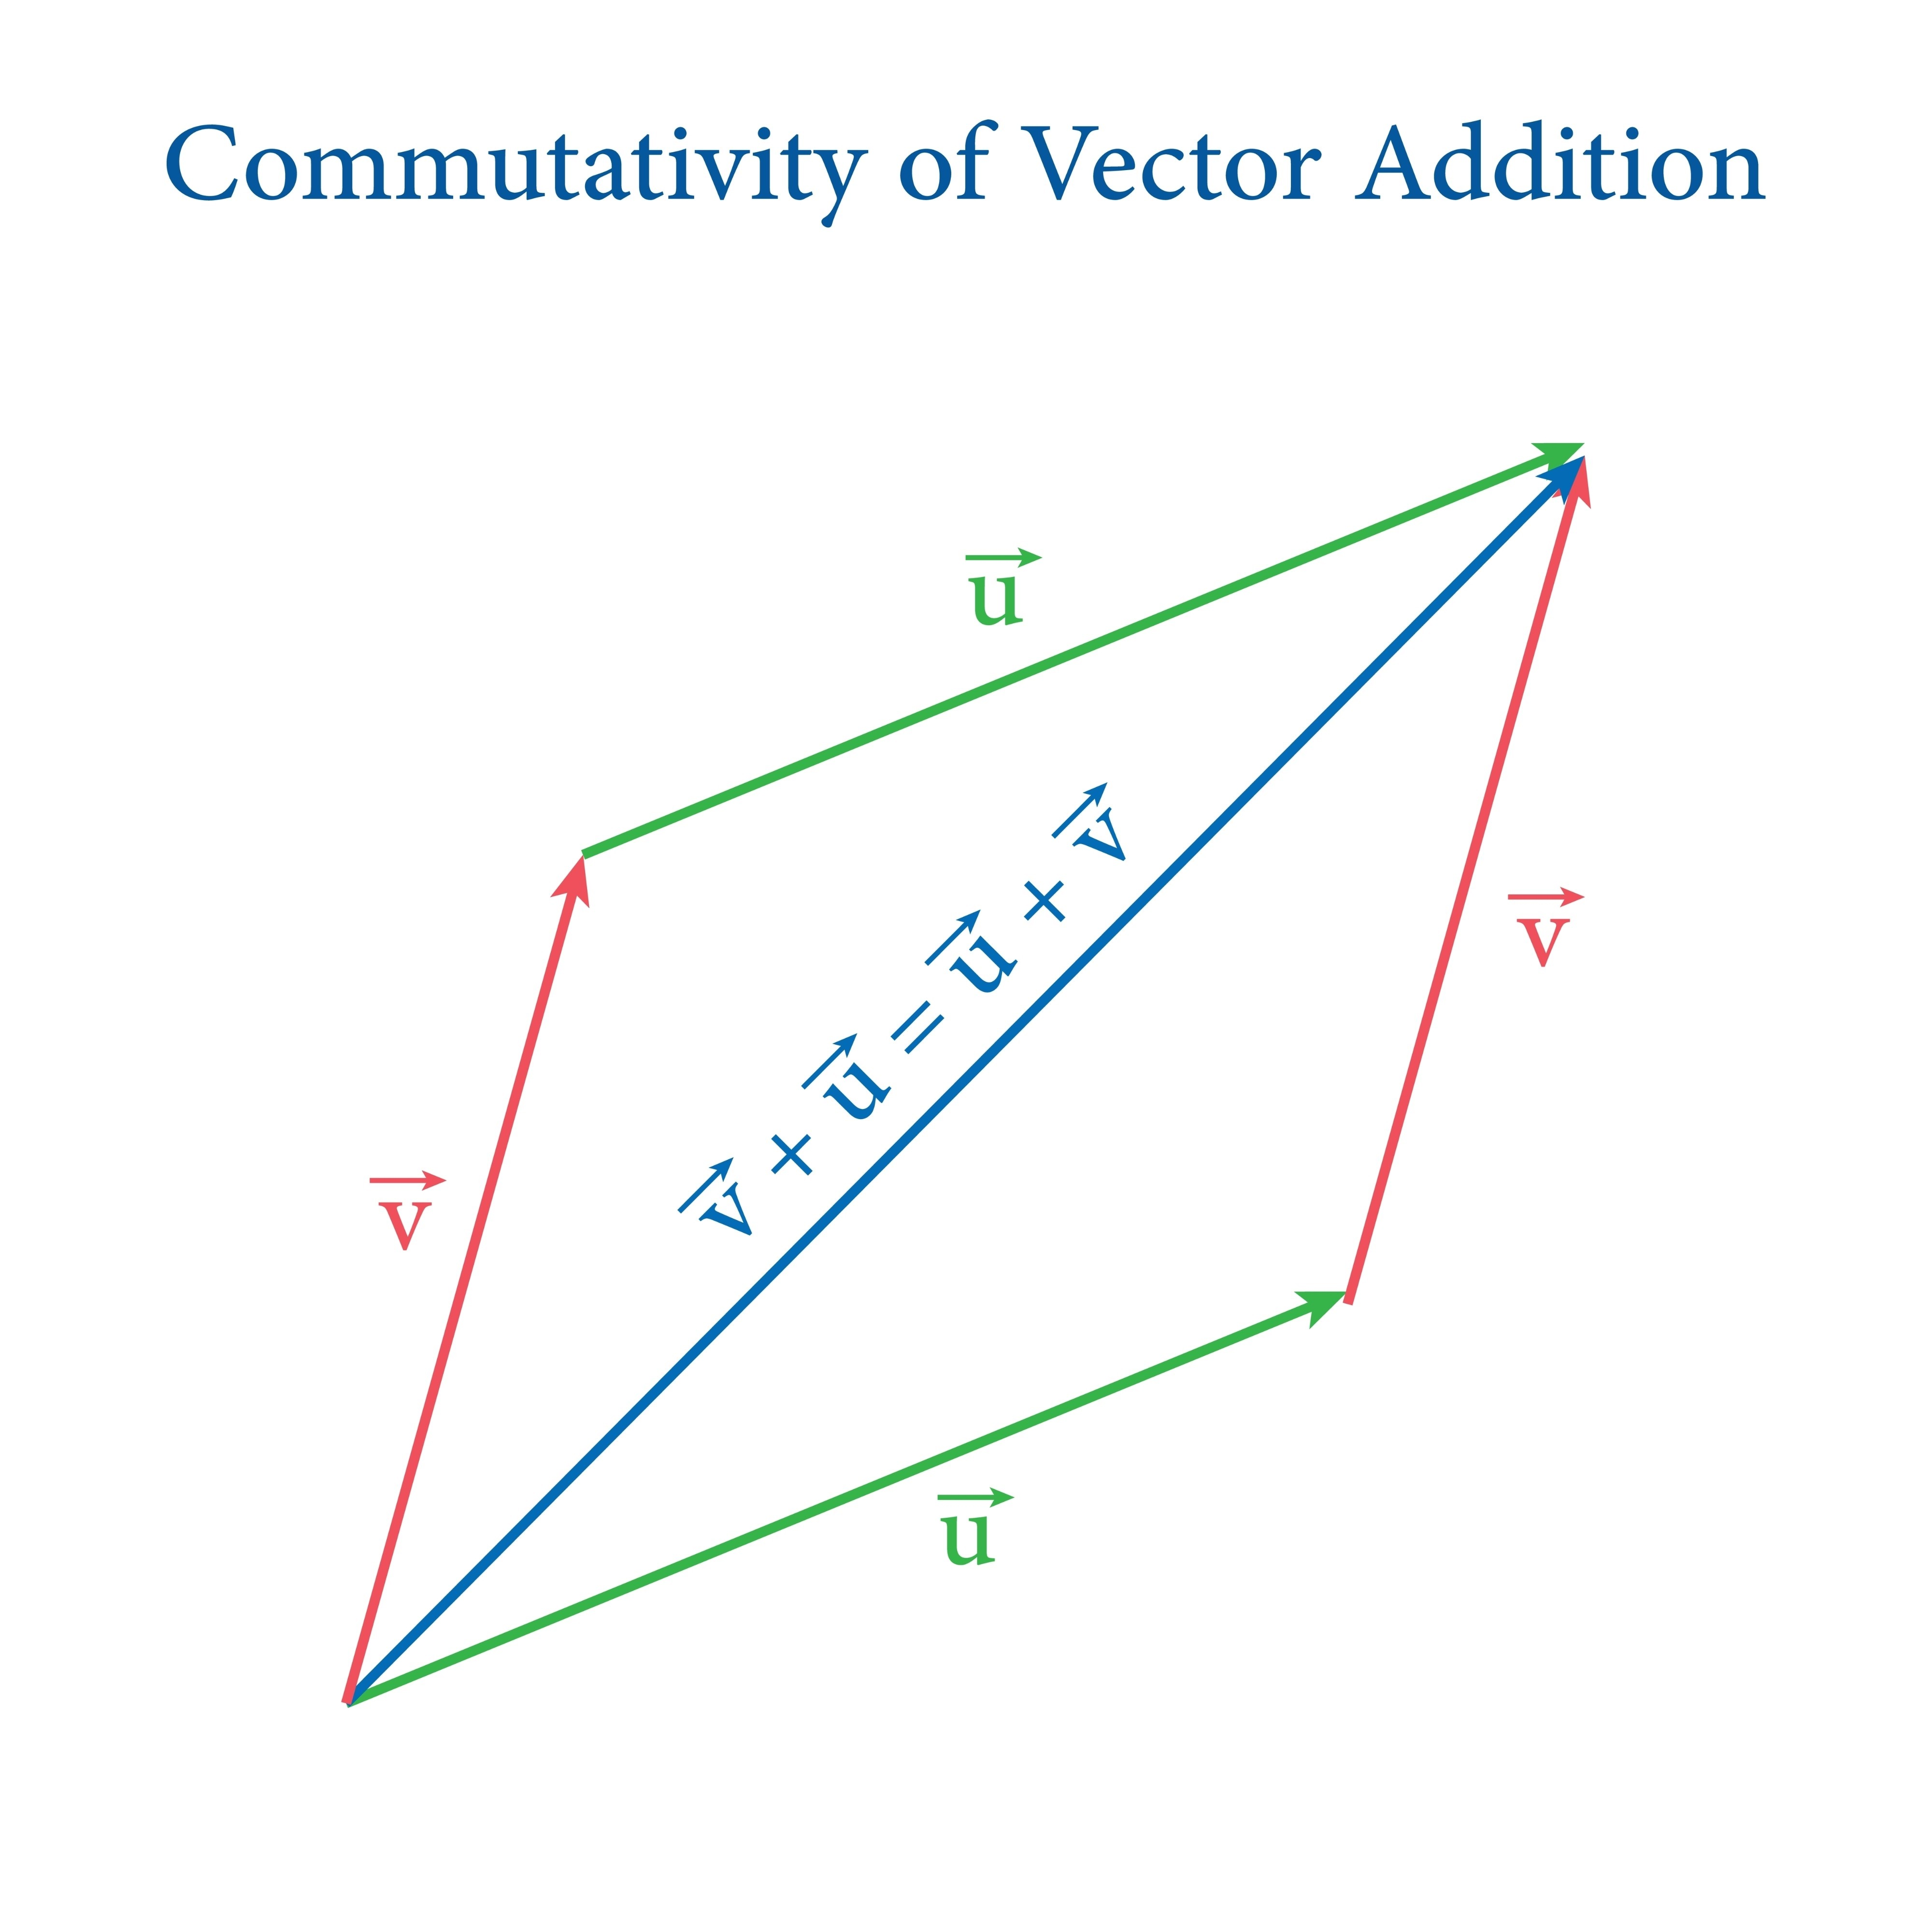
\includegraphics[width=0.55\textwidth]{figures/vector_addition.jpeg}
\caption{Visualizing vector addition.}
\end{figure}
\end{frame}

\begin{frame}[allowframebreaks]
\frametitle{Subspaces and Linear Mappings}
\begin{itemize}
    \item A subset $W$ of a vector space $V$ is a \textbf{subspace} if it is itself a vector space over the same scalar field, and $\vec{v}, \vec{w}\in W$ and $a, b \in \mathbb{F}$, $a\vec{v} + b\vec{w} \in W$
    \item A subspace is entirely contained within another vector space, written as $W \subset V$.
    \item A mapping $f: V \to W$ is a \textbf{linear mapping} if it preserves the structure of vector addition and scalar multiplication.
    \item Properties of linear mappings include:
    \begin{itemize}
        \item $f(\vec{x}+\vec{y})=f(\vec{x})+f(\vec{y})$.
        \item $f(a\vec{x})=af(\vec{x})$.
        \item $f(\vec{0}_{V})=\vec{0}_{W}$.
        \item $f(-\vec{x})=-f(\vec{x})$.
    \end{itemize}
\end{itemize}
\end{frame}

\begin{frame}[allowframebreaks]
\frametitle{Subspace Generation and Linear Dependence}
\begin{itemize}
    \item The set of all linear combinations of vectors $\{\vec{a}_1, \vec{a}_2, \dots, \vec{a}_n\}$ forms the smallest subspace containing these vectors. This is called the subspace \textbf{generated by} or \textbf{spanned by} the set.
    \item A set of vectors $A=\{\vec{a}_1, \vec{a}_2, \dots, \vec{a}_n\}$ is \textbf{linearly dependent} if there exist scalars $x_1, x_2, \dots, x_n$ (at least one of which is not zero) such that $x_{1}\vec{a}_{1}+x_{2}\vec{a}_{2}+\cdots+x_{n}\vec{a}_{n}=\vec{0}$.
    \item A set is \textbf{linearly independent} if the equation holds only when all scalars are zero ($x_1=x_2=\cdots=x_n=0$).
\end{itemize}
\end{frame}

\begin{frame}{Example}

    $\{2\vec{a}, 3\vec{a}\}$ for any vector $\vec{a}$ is linearly dependent because 

    $$
    3\cdot 2 \vec{a} + (-2)\cdot 3 \vec{a} = \vec{0}
    $$

    We choose $3$ and $-2$ to show that a linear combination of them may give zero vectors.
    
\end{frame}

\begin{frame}[containsverbatim]
\frametitle{Example 2: Linear Independence with SymPy}
\begin{itemize}
    \item To test for linear independence, you can solve the system of equations. For example, for $A = \{(1,2), (2,3)\} \subseteq \mathbb{R}^2$, the system is:
    
    \begin{multiequation}
        x \begin{bmatrix}
            1\\2
        \end{bmatrix} + y  \begin{bmatrix}
            2\\3
        \end{bmatrix} =  \begin{bmatrix}
            0\\0
        \end{bmatrix}
    \end{multiequation}
    \begin{align*}
        x+2y&=0 \\
        2x+3y&=0
    \end{align*}
    \item This system has a unique solution of $x=y=0$, so the set is linearly independent.
    \item We can use the \texttt{sympy} package in Python to solve this:
\end{itemize}
\begin{minted}[fontsize=\footnotesize]{python}
from sympy import solve
from sympy.abc import x, y
ans = solve([x + 2*y, 2*x + 3*y], [x, y])
print(ans)
\end{minted}
\end{frame}

\begin{frame}{Example 3}
    For $A = \{(1,2), (2,4)\} \subseteq \mathbb{R}^2$, the system is:

    \begin{multiequation}
        x + 2y & = 0\\
        2x + 4y = 0
    \end{multiequation}
    which has the solution $(x, y) = (2, -1)$ other than $(x, y) = (0, 0)$. Hence $A$ is not linearly dependent.

    \footnotesize
    \begin{tblock}{To Summarize:}
        Linear dependence of $A$ is equivalent to \textbf{there exists a vector in A that is linear combination of the other vectors of A}. The linear independence of $A$ is equivalent of \textbf{any vector in A never belongs to the subspace generated by the other vector but it}.
    \end{tblock}

\end{frame}

\begin{frame}[containsverbatim]
\frametitle{Basis and Dimension}
\begin{itemize}
    \item A set $X=\{\vec{a}_1, \dots, \vec{a}_n\}$ is a \textbf{basis} for a vector space V if it is both \textbf{linearly independent} and \textbf{generates V} (spans V).
    \item The \textbf{standard basis} for $\mathbb{R}^n$ is the set of vectors $\{\vec{e}_1, \vec{e}_2, \dots, \vec{e}_n\}$ where $\vec{e}_i$ has a 1 in the $i$-th position and 0s elsewhere.
    \item If a vector space V has a basis with $m$ vectors, then any other basis of V will also have $m$ vectors. This number $m$ is the \textbf{dimension} of V, denoted as $m = \text{dim}_{\mathbb{K}}V$.
    \item The dimension of the subspace generated by a set $A$ is called the \textbf{rank} of A, denoted as rank(A).
\end{itemize}
\end{frame}

\begin{frame}{Basis}

    Some points to note:
    \begin{enumerate}
    \item A set obtained by adding a new vector to $X$ or removing any vector of $X$ is no longer a basis of $V$.
    
    \item A set obtained by replacing any vector of $X$ with its nonzero scalar multiple remains a basis.
    
    \item A set obtained by replacing any vector of $X$ with a sum of it and a scalar multiple of another vector of $X$ remains a basis.
\end{enumerate}
    
\end{frame}

\begin{frame}{Standard Basis}
    The set $\{\vec{e}_1, \vec{e}_2, \ldots, \vec{e}_n\}$ is given by:
\begin{align}
\vec{e}_1 &= (1, 0, \ldots, 0) \\
\vec{e}_2 &= (0, 1, \ldots, 0) \\
&\vdots \\
\vec{e}_n &= (0, 0, \ldots, 1)
\end{align}

is a basis of $\mathbb{R}^n$. It is called as the \textbf{Standard basis}.

\vspace{0.5cm}

Let $X$ be the basis of $V$.

Assume that we serialize the vectors in $X$ as $\vec{a}_1, \vec{a}_2, \ldots, \vec{a}_n$ and fix this order.

For any vector $\vec{z} \in V$:
$$\vec{z} = x_1\vec{a}_1 + x_2\vec{a}_2 + \cdots + x_n\vec{a}_n$$

We call this \textcolor{blue}{the expansion of $\vec{z}$ on the basis of $X$}.

    
\end{frame}

\begin{frame}
\frametitle{Vector Representation}

The vector $\vec{x} = (x_1, x_2, \ldots, x_n) \in \mathbb{K}^n$ made of the expansion coefficient $x_1, x_2, \ldots, x_n$ is called \textcolor{blue}{the representation of $\vec{z}$ on the basis $X$}.

\vspace{0.5cm}

With the standard basis, we could write:
\begin{align}
\vec{x} &= x_1\vec{e}_1 + x_2\vec{e}_2 + \cdots + x_n\vec{e}_n \\
\vec{x} &= x_1(1,0,\ldots,0) + x_2(0,1,\ldots,0) + \cdots + x_n(0,0,\ldots,1)
\end{align}

\vspace{0.3cm}
\begin{tikzpicture}[overlay]
\node[draw, rounded corners, fill=yellow!20, text width=4cm, font=\scriptsize] at (8,-1) {
Note that at this point we are currently not caring about whether it is a column vector or row vector
};
\end{tikzpicture}

\end{frame}

\begin{frame}
\frametitle{Bijective Mapping Between Spaces}

$\ast$ $s\vec{z} + t\vec{y}$ implies $f_X(s\vec{z} + t\vec{y})$ where $f_X$ is bijective mapping from $V$ to $\mathbb{K}^n$

with 
$$f_X(s\vec{z} + t\vec{y}) = sf_X(\vec{z}) + tf_X(\vec{y})$$

\vspace{0.5cm}

\begin{tcolorbox}[colback=androidRedLight,colframe=red!50!black,title=Bijective mapping refresher:]
\begin{itemize}
    \item Every element in $\mathbb{K}^n$ is mapped to by exactly one element in $V$.
    \item Each element in $V$ maps to a unique element in $\mathbb{K}^n$.
\end{itemize}
\end{tcolorbox}

\end{frame}

\begin{frame}
\frametitle{Rank}

\textcolor{red}{\underline{Rank}}

The dimension of the subspace generated by $A = \{a_1, a_2, \ldots, a_n\}$ is called the \textbf{rank of $A$}. We denote it by $\text{rank}_\mathbb{K} A$ or $\text{rank } A$.

\vspace{0.5cm}

\textcolor{blue}{\underline{Some Points:}}
\begin{enumerate}
    \item $\text{rank } A \leq n$
    
    \item If $A$ is linearly independent, then $\text{rank } A = n$
    
    \item If $A$ is linearly dependent, then $\text{rank } A < n$
\end{enumerate}

\vspace{0.5cm}

If $A$ is a subset of an $m$-dimensional vector space $V$, then:
\begin{enumerate}
    \item $\text{rank } A \leq m$
    
    \item If $A$ generates $V$, then $\text{rank } A = m$.
    
    \item If $A$ doesn't generate $V$, then $\text{rank } A < m$.
\end{enumerate}

\end{frame}

\begin{frame}
\frametitle{Direct Sum}

\textcolor{red}{\underline{Direct Sum}}

Let $W_1, W_2, \ldots, W_k$ be subspaces of vector space $V$.

and $W = \{\vec{x}_1 + \vec{x}_2 + \cdots + \vec{x}_k \mid \vec{x}_1 \in W_1, \vec{x}_2 \in W_2, \ldots, \vec{x}_k \in W_k\}$

then $W$ is a subspace of $V$.

$W$ is called a \textbf{sum of subspaces}.

\vspace{0.5cm}

In this case, when every element $\vec{x}$ of $W$ is uniquely expressed $\vec{x} = \vec{x}_1 + \vec{x}_2 + \cdots + \vec{x}_k$ with $\vec{x}_1 \in W_1, \vec{x}_2 \in W_2, \ldots$ then we call $W$ the \textbf{direct sum} of $W_1, W_2, \ldots, W_k$.

\vspace{0.3cm}

We can also write $\mathbb{W} = \{W_1, W_2, \ldots, W_k\}$

and denote the direct sum as $W_1 \oplus W_2 \oplus \cdots \oplus W_k$.

\end{frame}

\begin{frame}[containsverbatim]
\frametitle{Python Implementation: Direct Sum}

\textcolor{androidRed}{In Python: direct sum can be written as}

\begin{minted}[fontsize=\small]{python}
[1, 2] + [3, 4, 5]
\end{minted}

Output: \texttt{[1, 2, 3, 4, 5]}

\vspace{0.3cm}

\textcolor{androidRed}{or using numpy}

\begin{minted}[fontsize=\small]{python}
from numpy import array, concatenate
concatenate (array([1,2]), array([3,4,5]))
\end{minted}

\vspace{0.3cm}

\textcolor{androidRed}{In sympy:}

\begin{minted}[fontsize=\small]{python}
from sympy import Matrix
Matrix([1,2]).col_join(Matrix([3,4,5]))
\end{minted}

\end{frame}

\begin{frame}[containsverbatim]
\frametitle{NumPy Arrays and n-Dimensional Arrangements}

We denote $n$-dimensional arrangement by arrays in NumPy Python.

\begin{enumerate}
    \item 1-D arrangement is a sequence of elements arranged in a row.
    
    \item 2D arrangement is a matrix in which elements are arranged vertically and horizontally in a 2-D plane.
    
    \item 3D arrangement is a layout of elements arranged vertically, horizontally, and depth-wise in 3D space.
\end{enumerate}

\vspace{0.5cm}


\begin{minted}[fontsize=\small]{python}
from numpy import array
A = array([1,2,3])                    # 1D
B = array([[1,2,3], [4,5,6]])         # 2D
C = array([[[1,2], [3,4]], [[5,6], [7,8]]])  #Two 2D Arrays
\end{minted}



\end{frame}

\begin{frame}[containsverbatim]
\frametitle{Vector Broadcasting in Python}

\small

Vector broadcasting is purely a computer operation.

Consider Python code:

\begin{minted}[fontsize=\small]{python}
v = np.array([[1,5,6]])    # row vector (2 columns)
w = np.array([[10,20,30]]).T    # column vector (3 rows)
v+w
\end{minted}

Output:

\begin{minted}[fontsize=\small]{python}
array([[11, 15, 16],
        [21, 25, 26],
        [31, 35, 36]])
\end{minted}

\textbf{What is going on?}

We are adding two vectors of dimension $1 \times 3$ and $3 \times 1$. Clearly there is a dimension mismatch but there doesn't seem to be an error!

Here, broadcasting operation is taking place even though there is a dimension mismatch.

\textcolor{blue}{Broadcasting essentially means to repeat an operation multiple times between one vector and each element of another vector.}

\end{frame}

\begin{frame}[fragile]
\frametitle{Example}

\begin{minted}{python}
import numpy as np
v = np.array([[1,2,3]]).T  # col vector 3 rows 1 col 3x1
w = np.array([[10,20]])    #  row vector 1 row 2 col 1x2
v+w
\end{minted}

It does the following operation on $v +w$:

\begin{multiequation}
~[1, 1] + [10, 20]\\
[2, 2] + [10, 20]\\
[3, 3] + [10, 20]
\end{multiequation}

\vspace{0.3cm}
Broadcasting allows for compact and efficient calculations in numerical coding.
\end{frame}


\section{Matrices}

\begin{frame}
    \sectionpage
\end{frame}

%------------------------------------------------
\begin{frame}{Matrices}
\begin{tblock}{Simplistic Definition:}
For a positive integer $m, n \in \Rbb$, a matrix $\Abf$ is $m\times n$ tuple of elements $a_{i, j}, i = 1, \cdot, m, j = 1, \cdot n $ which is ordered according to a rectangular scheme with $m$ rows and $n$ columns such that we can write:
\begin{multiequation}
    \label{eq:matrix}
        \Abf = \begin{bmatrix}
            a_{11} & a_{12} & a_{13} & \cdots & a_{1n}\\
            a_{21} & a_{22} & a_{23} & \cdots & a_{2n}\\
            \vdots & \vdots & \vdots & \cdots & \vdots\\
            a_{m1} & a_{m2} & a_{m3} & \cdots & a_{mn}\\
        \end{bmatrix}
\end{multiequation}
We will set a convention to use boldface uppercase letters to denote a matrix.
You can see that a matrix can be constructed by placing multiple row vectors or column vectors as well.
\end{tblock}
\end{frame}

%------------------------------------------------


\begin{frame}[containsverbatim]{Matrix in Python}
\begin{tblock}{A rectangular matrix}
\begin{minted}
[
framesep=1mm,
baselinestretch=1.2,
fontsize=\normalsize
]
{python}
import numpy as np
A = np.array([[1, 2, 3], [4, 5, 6]])
print(A.shape)
\end{minted}

Output:
\begin{minted}
[
framesep=1mm,
baselinestretch=1.2,
fontsize=\normalsize
]
{bash}
(2, 3)
\end{minted}
\end{tblock}

\end{frame}



%------------------------------------------------


\begin{frame}[containsverbatim]{Elementwise Matrix Multiplication (Hadamard Product)}
Two matrices with the same size can be multiplied together, and this is often called element-wise
matrix multiplication or the Hadamard product. It is denoted using a small circle $\circ$: $$\Cbf = \Abf\circ \Bbf$$.

\begin{tblock}{Hadamard Product}
\begin{minted}
[
framesep=1mm,
baselinestretch=1.2,
fontsize=\normalsize
]
{python}
import numpy as np
A = np.array([[1, 2, 3],[4, 5, 6]])
B = np.array([[1, 2, 3],[4, 5, 6]])
C = A * B
\end{minted}
\end{tblock}

\end{frame}

%------------------------------------------------
\begin{frame}[allowframebreaks, containsverbatim]{Matrix-Matrix Multiplication (Or, Matrix Multiplication)}

Matrix multiplication is a binary operation that takes a pair of  matrices and produces another matrix. If $\mathbf{A}$ is an $m \times n$ matrix and $\mathbf{B}$ is an $n \times k$ matrix, then their matrix product $\mathbf{AB}$ is an $m \times k$ matrix.

The element at the $i$-th row and $j$-th column of $\mathbf{C}$, denoted as $c_{ij}$, can be calculated as follows:

\begin{equation}
c_{ij} = \sum_{r=1}^{n} a_{ir}b_{rj}
\end{equation}

where $a_{ir}$ is the element at the $i$-th row and $r$-th column of $\mathbf{A}$, and $b_{rj}$ is the element at the $r$-th row and $j$-th column of $\mathbf{B}$. The summation runs over the $r$ index from 1 to $n$.


In Python, you can use the `numpy` library to perform matrix multiplication using the `dot` function.
\begin{tblock}{Matrix Multiplication}
\begin{minted}
[
framesep=1mm,
baselinestretch=1.2,
fontsize=\normalsize
]
{python}
import numpy as np
A = np.array([[1, 2], [3, 4]]) # 2x2 matrix
B = np.array([[5, 6], [7, 8]]) # 2x2 matrix
C = A.dot(B)
print(C)
\end{minted}

Output:
\begin{minted}
[
framesep=1mm,
baselinestretch=1.2,
fontsize=\normalsize
]
{bash}
[[19 22]
 [43 50]]
\end{minted}
\end{tblock}

\end{frame}

%------------------------------------------------

\begin{frame}[allowframebreaks, containsverbatim]{Types of Matrices}

\begin{tblock}{Triangular Matrices}
A triangular matrix is a special kind of square matrix where all the entries above the main diagonal are zero (lower triangular) or all the entries below the main diagonal are zero (upper triangular).

Example in Python:
\begin{minted}
[
framesep=1mm,
baselinestretch=1.2,
fontsize=\normalsize
]
{python}
import numpy as np
A = np.array([[1, 2, 3], [0, 4, 5], [0, 0, 6]]) # Upper triangular
B = np.array([[1, 0, 0], [4, 5, 0], [7, 8, 9]]) # Lower triangular
print("A = ", A)
print("B = ", B)
\end{minted}
\end{tblock}

\begin{tblock}{Identity Matrices}
An identity matrix $\Ibf$ is a square matrix in which all the elements of the principal diagonal are ones and all other elements are zeros.

Example in Python:
\begin{minted}
[
framesep=1mm,
baselinestretch=1.2,
fontsize=\normalsize
]
{python}
import numpy as np
I = np.eye(3) # 3x3 identity matrix
print("I = ", I)
\end{minted}
\end{tblock}

\begin{tblock}{Diagonal Matrices}
A diagonal matrix is a matrix in which the entries outside the main diagonal are all zero.

Example in Python:
\begin{minted}
[
framesep=1mm,
baselinestretch=1.2,
fontsize=\normalsize
]
{python}
import numpy as np
D = np.diag([1, 2, 3]) # Diagonal matrix with diagonal elements 1, 2, 3
print("D = ", D)
\end{minted}
\end{tblock}

\begin{tblock}{Orthogonal Matrices}
An orthogonal matrix is a square matrix whose rows and columns are orthogonal unit vectors (i.e., orthonormal vectors), making it a column and row-stochastic matrix. Orthogonal matrices have the property that their transpose is equal to their inverse, i.e.

$$
Q^\top = Q^{-1} \quad \text{or}\quad Q \cdot Q^\top = I
$$


\end{tblock}


\begin{tblock}{Orthogonal Matrices: Example in Python}

\begin{minted}
[
framesep=1mm,
baselinestretch=1.2,
fontsize=\normalsize
]
{python}
import numpy as np
Q = np.array([[1, 0], [0, -1]]) # An example of orthogonal matrix
print("Q = ", Q)
print("Q Transpose = ", Q.T)
print("Q Inverse = ", np.linalg.inv(Q))
\end{minted}
\end{tblock}

\end{frame}



\subsection{Operations on Matrices}

\begin{frame}
    \subsectionpage
\end{frame}

%------------------------------------------------

\begin{frame}[containsverbatim]{Operations on Matrices}

\begin{tblock}{Transpose}
The transpose of a matrix is obtained by interchanging its rows into columns or columns into rows. It is denoted by $\mathbf{A}^T$. For example, if 

\end{tblock}

\end{frame}

\begin{frame}[containsverbatim]{Operations on Matrices}



\begin{tblock}{Transpose: Example}


\begin{equation}
    A = \begin{pmatrix}
        1 & 2\\
        3 & 4\\
        5 & 6
    \end{pmatrix}
\end{equation}
then,
\begin{equation}
    A^\top = \begin{pmatrix}
        1 & 3 & 5\\
        2 & 4 & 6
    \end{pmatrix}
\end{equation}
\end{tblock}

\end{frame}

\begin{frame}[containsverbatim]{Operations on Matrices}


\begin{tblock}{Transpose: Example in Python}

\begin{minted}
[
framesep=1mm,
baselinestretch=1.2,
fontsize=\normalsize
]
{python}
import numpy as np
A = np.array([[1, 2, 3], [4, 5, 6]]) 
print("A = ", A)
print("Transpose of A = ", A.T)
\end{minted}
\end{tblock}

\end{frame}
\begin{frame}[containsverbatim]{Operations on Matrices}




\begin{tblock}{Determinant}
The determinant is a special number that can be calculated from a square matrix. The determinant helps us find the inverse of a matrix, tells us things about the matrix that are useful in systems of linear equations, calculus and more.

\end{tblock}

\end{frame}

\begin{frame}[containsverbatim]{Operations on Matrices}



\begin{tblock}{Determinant}

The determinant of a matrix gives us important information about the matrix. For example, a matrix is invertible (i.e., has an inverse) if and only if its determinant is non-zero. The determinant of a matrix also gives us the scale factor by which area (or volume, in higher dimensions) is transformed under the linear transformation represented by the matrix. 

It's important to note that the determinant is only defined for square matrices. For non-square matrices, related concepts like the rank or the pseudoinverse are often used instead.

\end{tblock}

\end{frame}

\begin{frame}[containsverbatim]{Operations on Matrices}


\begin{tblock}{A 2x2 Determinant}

The determinant of a matrix $\mathbf{A}$ is often denoted as $|\mathbf{A}|$ or $\text{det}(\mathbf{A})$.

For a 2x2 matrix:
$$
\mathbf{A} = \begin{bmatrix}
a & b \\
c & d
\end{bmatrix}
$$
The determinant is calculated as:
$$|\mathbf{A}| = ad - bc
$$
\end{tblock}

\end{frame}
\begin{frame}[containsverbatim]{Operations on Matrices}



\begin{tblock}{Determinant}
For a 3x3 matrix:
$$
\mathbf{A} = \begin{bmatrix}
a & b & c \\
d & e & f \\
g & h & i
\end{bmatrix}
$$
The determinant is calculated as:
$$|\mathbf{A}| = a(ei - fh) - b (di - gf) + c (dh - eg)
$$
For larger square matrices (4x4 and above), the determinant is usually computed using more advanced methods like the Laplace expansion, or LU decomposition. The determinant of a matrix can also be calculated using the product of its eigenvalues. 
\end{tblock}

\end{frame}

\begin{frame}[containsverbatim]{Operations on Matrices}



\begin{tblock}{Determinant: Example in Python}
\begin{minted}
[
framesep=1mm,
baselinestretch=1.2,
fontsize=\normalsize
]
{python}
A = np.array([[1, 2], [3, 4]])
print("A = ", A)
print("Determinant of A = ", np.linalg.det(A))
\end{minted}
\end{tblock}

\end{frame}
\begin{frame}[containsverbatim]{Operations on Matrices}



\begin{tblock}{Inverse}
The inverse of a square matrix $\mathbf{A}$ is denoted as $\mathbf{A}^{-1}$, and it is the matrix such that when it is multiplied by $\mathbf{A}$, the result is the identity matrix.

\textbf{Example in Python:}
\begin{minted}
[
framesep=1mm,
baselinestretch=1.2,
fontsize=\normalsize
]
{python}
A = np.array([[4, 7], [2, 6]])
print("A = ", A)
print("Inverse of A = ", np.linalg.inv(A))
\end{minted}
\end{tblock}

\end{frame}
\begin{frame}[containsverbatim]{Operations on Matrices}



\begin{tblock}{Trace}
The trace of a square matrix $\mathbf{A}$, denoted as $\text{tr}(\mathbf{A})$, is the sum of the elements on the main diagonal.

\textbf{Example in Python:}
\begin{minted}
[
framesep=1mm,
baselinestretch=1.2,
fontsize=\normalsize
]
{python}
A = np.array([[1, 2], [3, 4]])
print("A = ", A)
print("Trace of A = ", np.trace(A))
\end{minted}
\end{tblock}

\end{frame}

\begin{frame}[containsverbatim]{Operations on Matrices}



\begin{tblock}{Rank}
The rank of a matrix $\mathbf{A}$ is the maximum number of linearly independent row vectors in the matrix.

Example in Python:
\begin{minted}
[
framesep=1mm,
baselinestretch=1.2,
fontsize=\normalsize
]
{python}
A = np.array([[1, 2, 3], [4, 5, 6], [7, 8, 9]])
print("A = ", A)
print("Rank of A = ", np.linalg.matrix_rank(A))
\end{minted}
\end{tblock}

\end{frame}


\subsection{Applications of Matrices}

\begin{frame}
    \subsectionpage
\end{frame}


% \begin{frame}{LU Decomposition}

%     \begin{tblock}{}
%         Factor a matrix $A$ into two triangle matrices: a lower triangle ($L$), an upper triangle matrix ($U$):
        
%         $$
%         A = LU = \begin{pmatrix}
% l_{11} & 0 & \cdots & 0 \\
% l_{21} & l_{22} & \cdots & 0 \\
% \vdots & \vdots & \ddots & \vdots \\
% l_{n1} & l_{n2} & \cdots & l_{nn}
% \end{pmatrix}
% \begin{pmatrix}
% u_{11} & u_{12} & \cdots & u_{1n} \\
% 0 & u_{22} & \cdots & u_{2n} \\
% \vdots & \vdots & \ddots & \vdots \\
% 0 & 0 & \cdots & u_{nn}
% \end{pmatrix}
%         $$
%     \end{tblock}

%     \textbf{Why?}

%     \bigskip

%     Reduce computational cost for many numerical problems.
    
% \end{frame}

\begin{frame}{Solving Systems of Linear Equations}
    \footnotesize
    Let's look at the systems of linear equations again.
    \begin{tblock}{}   
\begin{multiequation}\label{eq:syslinearcomb2}
    a_{11}x_1 + a_{12}x_2 + \cdots + a_{1n}x_n & = b_1\\
    a_{21}x_1 + a_{22}x_2 + \cdots + a_{2n}x_n & = b_2\\
    \vdots\\
    a_{m1}x_1 + a_{m2}x_2 + \cdots + a_{mn}x_n & = b_m\\
    a_{ij}, b_{i}\in \mathbb{R}
\end{multiequation}
\end{tblock}

In Matrix form, we could write it as 
\begin{multiequation}
    \begin{bmatrix}
        a_{11} & a_{12} & \cdots & a_{1n}\\
        a_{21} & a_{22} & \cdots & a_{2n}\\
        \cdots & \cdots & \cdots & \cdots\\
        a_{m1} & a_{m2} & \cdots & a_{mn}
    \end{bmatrix}_{m\times n}
    \begin{bmatrix}
        x_1\\
        x_2\\
        \vdots\\
        x_{n}
    \end{bmatrix}_{n\times 1} &= \begin{bmatrix}
        b_1\\
        b_2\\
        \vdots\\
        b_{m}
    \end{bmatrix}_{m\times 1}\\
    A_{m\times n} X_{n\times 1} = B_{m\times 1}
\end{multiequation}

\end{frame}


\begin{frame}{How to Solve Systems of Linear Equations using Matrix}
    
    \begin{multiequation}
        AX & = B
    \end{multiequation}

    \begin{enumerate}
        \item Matrix Inverse
        \item Gaussian Elimination
    \end{enumerate}

\end{frame}

\begin{frame}{Matrix Inverse}


    \begin{columns}
        \column{0.5\linewidth}
        \begin{tblock}{}
        \begin{multiequation}
        X = A^{-1}B
    \end{multiequation}
    \end{tblock}

    \column{0.5\linewidth}
        Inverse can be calculated as

            \begin{tblock}{}
        \begin{multiequation}
        A^{-1} = \cfrac{1}{|A|}Adj A
    \end{multiequation}
    \end{tblock}
    where $|A|$ is the determininant of the matrix.

    \bigskip

    $Adj(A)$ is the adjoint of a matrix $A$ (not the same as a adjoint Matrix. $adj(A)$ is also called adjugate matrix.


    \end{columns}    
\end{frame}

\begin{frame}{Example}

    Consider $ A = \begin{bmatrix}
        -2 & 5 & 1\\
        4 & 1 & 0\\
        -3 & 5 & 5
    \end{bmatrix}$. $Adj(A)$ can be written as $Adj(A) = \begin{bmatrix}
        C_{11} & C_{2} & C_{31}\\
        C_{12} & C_{22} & C_{23}\\
        C_{13} & C_{23} & C_{33}
    \end{bmatrix}$. $C_{ij}$ are called cofactors.

    \bigskip

    $C_{11} = + \bigg|  \begin{bmatrix}
        1 & 0 \\
        5 & 5
    \end{bmatrix} \bigg| = 5 - 0 = 5$, ~~~ $C_{12} = - \bigg|  \begin{bmatrix}
        4 & 0 \\
        -3 & 5
    \end{bmatrix} \bigg| = -(20 - 0 ) = -20$, $C_{13} = + \bigg|  \begin{bmatrix}
        4 & 1 \\
        -3 & 5
    \end{bmatrix} \bigg| = 20 + 3  = 23$. Similarly, you can calculate for $C_{ij}$. \bigskip This way, $Adj(A) = \begin{bmatrix}
        5 & -20 & -1\\-20 & -7 & 4\\23 & -5 & -22
    \end{bmatrix}$
    
\end{frame}

\begin{frame}{General Formula for Solving Systems of Linear Equations by Inverse}
    \begin{enumerate}
        \item First, calculate the cofactors $C_{ij} = (-1)^{i+j} M_{ij}$ where $M_{ij}$ is the determininant of $(n-1) \times (n-1)$ matrix resulting from deleting row $i$ and column $j$ of $A$.
        \item Divide cofactor matrix by $det(A) = |A|$.
    \end{enumerate}

    \begin{multiequation}
        AX & = B\\
        A^{-1}A X & = A^{-1}B\\
        IX & = A^{-1}B\\
        X & = A^{-1}B
    \end{multiequation}

    \begin{block}{}
        \faExclamationTriangle~~~Computing $Adj(A)$ for a high-dimensional matrix is computationally expensive. We need better methods.
    \end{block}

    We use Gaussian elimination method for solving large matrices. For that we need to understand Row Echelon Form, and elementary operations.
\end{frame}

\begin{frame}{What is Row Echelon Form?}

\begin{block}{}
    \centering
    A matrix is in \alert{Row Echelon Form (REF)} if it satisfies these rules:
\end{block}

\vspace{5mm}
\begin{enumerate}
    \item \textbf{Leading Entry Rule:} Any non-zero row has a leading \alert{\textbf{1}} (pivot)
    \item \textbf{Staircase Rule:} Each pivot is \alert{right} of the one above
    \item \textbf{Zero Rule:} All-zero rows are at the \alert{bottom}
\end{enumerate}

\centering

\vspace{5mm}
$\begin{bmatrix}
\alert{\mathbf{1}} & 2 & 3 & 4 \\
0 & \alert{\mathbf{1}} & 5 & 6 \\
0 & 0 & 0 & \alert{\mathbf{1}} \\
\end{bmatrix}$
\hspace{10mm}
$\begin{bmatrix}
\alert{\mathbf{1}} & 2 & 3 \\
0 & 0 & \alert{\mathbf{1}} \\
0 & 0 & 0 \\
\end{bmatrix}$
\end{frame}

\begin{frame}{Elementary Row Operations}
\centering
We use these operations to achieve REF:

\vspace{5mm}
\begin{tabular}{lll}
\toprule
\textbf{Operation} & \textbf{Notation} & \textbf{Effect} \\
\midrule
Row Swap & $R_i \leftrightarrow R_j$ & Swap two rows \\
Scaling & $kR_i$ & Multiply row by non-zero $k$ \\
Replacement & $R_i + kR_j$ & Add multiple of one row to another \\
\bottomrule
\end{tabular}

\vspace{8mm}
\alert{Key Property:} These operations do \textbf{not} change the solution set of the system!
\end{frame}

\begin{frame}{Step-by-Step Example: Starting Matrix}
\centering
Let's transform this matrix into REF:

$$
A = \begin{bmatrix}
0 & 3 & -6 & 6 & 4 \\
3 & -7 & 8 & -5 & 8 \\
3 & -9 & 12 & -9 & 6 \\
\end{bmatrix}
$$

\vspace{5mm}
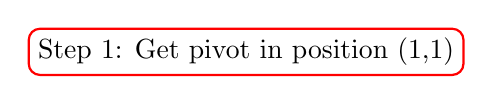
\begin{tikzpicture}
\node[draw=red, rounded corners, thick] {Step 1: Get pivot in position (1,1)};
\end{tikzpicture}
\end{frame}

\begin{frame}{Step 1: Create First Pivot}
\centering
Swap Rows 1 and 2, then scale new Row 1:

\vspace{3mm}
$R_1 \leftrightarrow R_2$ then $\frac{1}{3}R_1$


\vspace{3mm}
$$
\rightarrow \begin{bmatrix}
\alert{\mathbf{1}} & -\frac{7}{3} & \frac{8}{3} & -\frac{5}{3} & \frac{8}{3} \\
0 & 3 & -6 & 6 & 4 \\
3 & -9 & 12 & -9 & 6 \\
\end{bmatrix}
$$
\end{frame}


\begin{frame}{Step 2: Create Zeros Below Pivot}
\centering
Eliminate the 3 in position (3,1):

\vspace{3mm}
$-3R_1 + R_3$

\vspace{3mm}
$$
\rightarrow \begin{bmatrix}
\alert{\mathbf{1}} & -\frac{7}{3} & \frac{8}{3} & -\frac{5}{3} & \frac{8}{3} \\
0 & 3 & -6 & 6 & 4 \\
\alert{\mathbf{0}} & -2 & 4 & -4 & -2 \\
\end{bmatrix}
$$
\end{frame}

\begin{frame}{Step 3: Create Second Pivot}
\centering
Scale Row 2 to create pivot:

\vspace{3mm}
$\frac{1}{3}R_2$

\vspace{3mm}
$$
\rightarrow \begin{bmatrix}
\alert{\mathbf{1}} & -\frac{7}{3} & \frac{8}{3} & -\frac{5}{3} & \frac{8}{3} \\
0 & \alert{\mathbf{1}} & -2 & 2 & \frac{4}{3} \\
0 & -2 & 4 & -4 & -2 \\
\end{bmatrix}
$$
\end{frame}

\begin{frame}{Step 4: Create More Zeros}
\centering
Eliminate below second pivot:

\vspace{3mm}
$2R_2 + R_3$

\vspace{3mm}
$$
\rightarrow \begin{bmatrix}
\alert{\mathbf{1}} & -\frac{7}{3} & \frac{8}{3} & -\frac{5}{3} & \frac{8}{3} \\
0 & \alert{\mathbf{1}} & -2 & 2 & \frac{4}{3} \\
0 & \alert{\mathbf{0}} & 0 & 0 & \frac{2}{3} \\
\end{bmatrix}
$$
\end{frame}

\begin{frame}{Step 5: Final REF Form}
\centering
Scale Row 3 for final pivot:

\vspace{3mm}
$\frac{3}{2}R_3$

\vspace{3mm}
$$
A_{\text{REF}} = \begin{bmatrix}
\alert{\mathbf{1}} & -\frac{7}{3} & \frac{8}{3} & -\frac{5}{3} & \frac{8}{3} \\
0 & \alert{\mathbf{1}} & -2 & 2 & \frac{4}{3} \\
0 & 0 & 0 & 0 & \alert{\mathbf{1}} \\
\end{bmatrix}
$$

\vspace{3mm}
\alert{Success!} Matrix is now in Row Echelon Form.
\end{frame}


\begin{frame}{Calculating Matrix Inverse}

    
To find the inverse $A^{-1}$ of a matrix $A$, we need to solve:
$$
A X = I_n
$$
for the unknown matrix $X$, which will be $A^{-1}$.

\vspace{5mm}
We can set this up as an \alert{Augmented Matrix}:
$$
\left[A \mid I_n \right]
$$

\vspace{3mm}
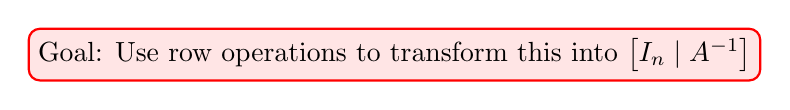
\begin{tikzpicture}
\node[draw=red, rounded corners, thick, fill=red!10] {Goal: Use row operations to transform this into $\left[I_n \mid A^{-1} \right]$};
\end{tikzpicture}

\vspace{3mm}
The process is Gaussian Elimination (also called Gauss-Jordan Elimination), and we perform the operations on the entire augmented matrix.
\end{frame}

\begin{frame}{Reduced Row Echelon Form}
An equation system is in reduced REF if
    \begin{enumerate}
        \item It is in REF.
        \item Every pivot is 1.
        \item The pivot is the only non-zero entry in its column.
    \end{enumerate}

    \alert{Example:}

    \centering
    $$
    A = \begin{bmatrix}
        1 & 3 & 0 & 0 & 3\\
        0 & 0 & 1 & 0 & 9\\
        0 & 0 & 0 & 1 & -4
    \end{bmatrix}
    $$
    
\end{frame}

\begin{frame}{Example: Matrix $A$ and Its Augmented Matrix}
    \footnotesize
\centering
$$
A = \begin{bmatrix}
1 & 0 & 2 & 0 \\
1 & 1 & 0 & 0 \\
1 & 2 & 0 & 1 \\
1 & 1 & 1 & 1 \\
\end{bmatrix}
$$

\vspace{3mm}
We form the augmented matrix $[A | I_4]$:

$$
\left[\begin{array}{cccc|cccc}
1 & 0 & 2 & 0 & 1 & 0 & 0 & 0 \\
1 & 1 & 0 & 0 & 0 & 1 & 0 & 0 \\
1 & 2 & 0 & 1 & 0 & 0 & 1 & 0 \\
1 & 1 & 1 & 1 & 0 & 0 & 0 & 1 \\
\end{array}\right]
$$

\vspace{3mm}
Our goal is to turn the left side into $I_4$. The right side will then become $A^{-1}$. We need to use eleme matrix operation to convert left side to reduce REF.
\end{frame}


\begin{frame}{Step 1: Establish the First Pivot}
    \footnotesize

\centering
Pivot position (1,1) is already \alert{1}. Now, we create zeros below it.

\vspace{3mm}
Operations:
\begin{align*}
R_2 &= R_2 - R_1 \\
R_3 &= R_3 - R_1 \\
R_4 &= R_4 - R_1
\end{align*}

\vspace{3mm}
$$
\rightarrow \left[\begin{array}{cccc|cccc}
1 & 0 & 2 & 0 & 1 & 0 & 0 & 0 \\
0 & 1 & -2 & 0 & -1 & 1 & 0 & 0 \\
0 & 2 & -2 & 1 & -1 & 0 & 1 & 0 \\
0 & 1 & -1 & 1 & -1 & 0 & 0 & 1 \\
\end{array}\right]
$$

\vspace{3mm}
\colorbox{red!20}{Pivot: position (1,1) = 1} \\
\colorbox{blue!20}{Zeros created below pivot in column 1}
\end{frame}


\begin{frame}{Step 2: Establish the Second Pivot}
    \footnotesize
\centering
Pivot position (2,2) is already \alert{1}. Create zeros above and below it.

\vspace{3mm}
Operations:
\begin{align*}
R_3 &= R_3 - 2R_2 \\
R_4 &= R_4 - R_2
\end{align*}

\vspace{3mm}
$$
\rightarrow \left[\begin{array}{cccc|cccc}
1 & 0 & 2 & 0 & 1 & 0 & 0 & 0 \\
0 & 1 & -2 & 0 & -1 & 1 & 0 & 0 \\
0 & 0 & 2 & 1 & 1 & -2 & 1 & 0 \\
0 & 0 & 1 & 1 & 0 & -1 & 0 & 1 \\
\end{array}\right]
$$

\vspace{3mm}
\colorbox{red!20}{Pivots: positions (1,1) = 1 and (2,2) = 1} \\
\colorbox{blue!20}{Zeros created below pivot in column 2}
\end{frame}

\begin{frame}{Step 3: Establish the Third Pivot}
        \footnotesize
\centering
Pivot position (3,3) is \alert{2}. Scale Row 3 to make it \alert{1}.

\vspace{3mm}
Operation:
$$
R_3 = \frac{1}{2} R_3
$$

\vspace{3mm}
$$
\rightarrow \left[\begin{array}{cccc|cccc}
1 & 0 & 2 & 0 & 1 & 0 & 0 & 0 \\
0 & 1 & -2 & 0 & -1 & 1 & 0 & 0 \\
0 & 0 & 1 & 0.5 & 0.5 & -1 & 0.5 & 0 \\
0 & 0 & 1 & 1 & 0 & -1 & 0 & 1 \\
\end{array}\right]
$$

\vspace{3mm}
Now create zeros above and below the new pivot.
\vspace{3mm}
Operations:
\begin{align*}
R_1 &= R_1 - 2R_3 \\
R_2 &= R_2 + 2R_3 \\
R_4 &= R_4 - R_3
\end{align*}
\end{frame}

\begin{frame}{Step 3 (Cont'd): Results after Eliminations}
            \footnotesize
\centering
$$
\rightarrow \left[\begin{array}{cccc|cccc}
1 & 0 & 0 & -1 & 0 & 2 & -1 & 0 \\
0 & 1 & 0 & 1 & 0 & -1 & 1 & 0 \\
0 & 0 & 1 & 0.5 & 0.5 & -1 & 0.5 & 0 \\
0 & 0 & 0 & 0.5 & -0.5 & 0 & -0.5 & 1 \\
\end{array}\right]
$$

\vspace{3mm}
\colorbox{red!20}{Pivots: positions (1,1), (2,2), (3,3) = 1} \\
\colorbox{blue!20}{Zero created below pivot in column 3}
\end{frame}

\begin{frame}{Step 4: Establish the Fourth Pivot}
            \footnotesize
\centering
Pivot position (4,4) is \alert{0.5}. Scale Row 4 to make it \alert{1}.

\vspace{3mm}
Operation:
$$
R_4 = 2 R_4
$$

\vspace{3mm}
$$
\rightarrow \left[\begin{array}{cccc|cccc}
1 & 0 & 0 & -1 & 0 & 2 & -1 & 0 \\
0 & 1 & 0 & 1 & 0 & -1 & 1 & 0 \\
0 & 0 & 1 & 0.5 & 0.5 & -1 & 0.5 & 0 \\
0 & 0 & 0 & 1 & -1 & 0 & -1 & 2 \\
\end{array}\right]
$$

\vspace{3mm}
Now create zeros above the new pivot.
\vspace{3mm}
Operations:
\begin{align*}
R_1 &= R_1 + R_4 \\
R_2 &= R_2 - R_4 \\
R_3 &= R_3 - 0.5R_4
\end{align*}
\end{frame}

\begin{frame}{Step 4 (Cont'd): The Final Result - Reduced Row Echelon Form}
\centering
After performing the final eliminations, we achieve our goal:

\vspace{3mm}
$$
\left[\begin{array}{cccc|cccc}
1 & 0 & 0 & 0 & -1 & 2 & -2 & 2 \\
0 & 1 & 0 & 0 & 1 & -1 & 2 & -2 \\
0 & 0 & 1 & 0 & 1 & -1 & 1 & -1 \\
0 & 0 & 0 & 1 & -1 & 0 & -1 & 2 \\
\end{array}\right]
$$

\vspace{5mm}
\fcolorbox{red}{red!10}{\parbox{0.7\textwidth}{\centering
Success! The left side is $I_4$. \\
Therefore, the right side is $\mathbf{A^{-1}}$}}
\end{frame}

\begin{frame}{We Have Found the Inverse!}
\centering
We can now read off the inverse matrix from the augmented matrix:

\vspace{5mm}
$$
A^{-1} = \begin{bmatrix}
-1 & 2 & -2 & 2 \\
1 & -1 & 2 & -2 \\
1 & -1 & 1 & -1 \\
-1 & 0 & -1 & 2 \\
\end{bmatrix}
$$

\vspace{5mm}
\begin{block}{Verification}
We can verify this is correct by checking that $A \cdot A^{-1} = I_4$. Multiplying the original matrix $A$ by this found matrix $A^{-1}$ will indeed yield the identity matrix. Using this, we can find the solution of a system of linear equations.
\end{block}
\end{frame}

\begin{frame}{Solving A System of Linear Equations Directly with Gaussian Elimination}

    Consider a system of linear equations as 

    \begin{multiequation}
        2x_1 + 3x_2 + 5x_3 & = 1\\
        4x_1 - 2x_2 - 7x_3 & = 8\\
        9x_1 + 5x_2 - 3x_3 & = 2
    \end{multiequation}
    
    We can write augmented matrix as 

    $$
\left[\begin{array}{ccc|c}
2 & 3 & 5 & 1\\
4 & -2 & -7 & 8\\
9 & 5 & -3 & 2
\end{array}\right]
$$

\end{frame}

\begin{frame}{Step 1: Goal for Column 1}
\centering
\textbf{Goal:} Get a pivot of \alert{1} in position (1,1) and zeros below it.

$$
\left[\begin{array}{ccc|c}
2 & 3 & 5 & 1\\
4 & -2 & -7 & 8\\
9 & 5 & -3 & 2
\end{array}\right]
$$

\vspace{5mm}
\textbf{Strategy:}
\begin{enumerate}
    \item First, make the pivot \textbf{1} by scaling Row 1.
    \item Then, eliminate the entries below it (4 and 9).
\end{enumerate}
\end{frame}

\begin{frame}{Step 1a: Create the First Pivot}
\centering
Scale Row 1 by $\frac{1}{2}$ to get a \alert{1} in position (1,1).

\vspace{3mm}
\alert{Operation:} $R_1 = \frac{1}{2} R_1$

\vspace{3mm}
$$
\rightarrow \left[\begin{array}{ccc|c}
1 & 1.5 & 2.5 & 0.5\\
4 & -2 & -7 & 8\\
9 & 5 & -3 & 2
\end{array}\right]
$$

\vspace{3mm}
\colorbox{red!20}{Pivot created at position (1,1) = 1}
\end{frame}

\begin{frame}{Step 1b: Eliminate Below the First Pivot}
\centering
Use the new pivot to create \alert{zeros} in the rest of column 1.

\vspace{3mm}
\alert{Operations:}
\begin{align*}
R_2 &= R_2 - 4R_1 \\
R_3 &= R_3 - 9R_1
\end{align*}

\vspace{3mm}
$$
\rightarrow \left[\begin{array}{ccc|c}
1 & 1.5 & 2.5 & 0.5\\
0 & -8 & -17 & 6\\
0 & -8.5 & -25.5 & -2.5
\end{array}\right]
$$

\vspace{3mm}
\colorbox{red!20}{Pivot: position (1,1) = 1} \\
\colorbox{blue!20}{Zeros created below pivot in column 1}
\end{frame}

\begin{frame}{Step 2: Goal for Column 2}
\centering
\textbf{Goal:} Get a pivot of \alert{1} in position (2,2) and zeros below it.

$$
\left[\begin{array}{ccc|c}
1 & 1.5 & 2.5 & 0.5\\
0 & -8 & -17 & 6\\
0 & -8.5 & -25.5 & -2.5
\end{array}\right]
$$

\vspace{5mm}
\textbf{Strategy:}
\begin{enumerate}
    \item First, make the pivot \textbf{1} by scaling Row 2.
    \item Then, eliminate the entry below it (-8.5).
\end{enumerate}
\end{frame}

\begin{frame}{Step 2a: Create the Second Pivot}
\centering
Scale Row 2 by $-\frac{1}{8}$ to get a \alert{1} in position (2,2).

\vspace{3mm}
\alert{Operation:} $R_2 = -\frac{1}{8} R_2$

\vspace{3mm}
$$
\rightarrow \left[\begin{array}{ccc|c}
1 & 1.5 & 2.5 & 0.5\\
0 & 1 & 2.125 & -0.75\\
0 & -8.5 & -25.5 & -2.5
\end{array}\right]
$$

\vspace{3mm}
\colorbox{red!20}{Pivots: positions (1,1) = 1 and (2,2) = 1}
\end{frame}

\begin{frame}{Step 2b: Eliminate Below the Second Pivot}
\centering
Use the new pivot to create a \alert{zero} in the rest of column 2.

\vspace{3mm}
\alert{Operation:}
$R_3 = R_3 + 8.5R_2$

\vspace{3mm}
$$
\rightarrow \left[\begin{array}{ccc|c}
1 & 1.5 & 2.5 & 0.5\\
0 & 1 & 2.125 & -0.75\\
0 & 0 & -7.4375 & -8.875
\end{array}\right]
$$

\vspace{3mm}
\colorbox{red!20}{Pivots: positions (1,1) and (2,2) = 1} \\
\colorbox{blue!20}{Zero created below pivot in column 2}
\end{frame}

\begin{frame}{Step 3: Goal for Column 3 \& Back-Substitution}
\centering
\textbf{Goal:} Get a pivot of \alert{1} in position (3,3). The matrix is now in Row Echelon Form (REF). We can then use \alert{back-substitution} to solve.

$$
\left[\begin{array}{ccc|c}
1 & 1.5 & 2.5 & 0.5\\
0 & 1 & 2.125 & -0.75\\
0 & 0 & -7.4375 & -8.875
\end{array}\right]
$$

\vspace{5mm}
\textbf{Strategy:}
\begin{enumerate}
    \item Scale Row 3 to get the final pivot.
    \item Read the simplified system from the REF matrix.
    \item Solve from the bottom up.
\end{enumerate}
\end{frame}

\begin{frame}{Step 3a: Create the Third Pivot}
\centering
Scale Row 3 by $-\frac{1}{7.4375}$ to get a \alert{1} in position (3,3).\\ (Note: $-\frac{1}{7.4375} \approx -0.1345$)

\vspace{3mm}
\alert{Operation:} $R_3 = -\frac{1}{7.4375} R_3$

\vspace{3mm}
$$
\rightarrow \left[\begin{array}{ccc|c}
1 & 1.5 & 2.5 & 0.5\\
0 & 1 & 2.125 & -0.75\\
0 & 0 & 1 & 1.193
\end{array}\right]
$$

\vspace{3mm}
\colorbox{red!20}{All pivots: positions (1,1), (2,2), (3,3) = 1}
\end{frame}

\begin{frame}{Step 4: Back-Substitution}
\centering
The REF matrix corresponds to the simplified system:

\vspace{3mm}
\begin{align*}
x_1 + 1.5x_2 + 2.5x_3 &= 0.5 \\
x_2 + 2.125x_3 &= -0.75 \\
x_3 &= 1.193
\end{align*}

\vspace{5mm}
\textbf{Solve from the bottom up:}
\begin{enumerate}
    \item From Eq. 3: \alert{$x_3 = 1.193$}
    \item Substitute $x_3$ into Eq. 2: $x_2 = -0.75 - 2.125(1.193) \approx -3.285$
    \item Substitute $x_2, x_3$ into Eq. 1: $x_1 = 0.5 - 1.5(-3.285) - 2.5(1.193) \approx 2.445$
\end{enumerate}

\vspace{3mm}
\begin{block}{Solution}
$\mathbf{x_1 \approx 2.445, \quad x_2 \approx -3.285, \quad x_3 \approx 1.193}$
\end{block}
\end{frame}

\section{Eigenvalues and Eigenvectors}

\begin{frame}
    \sectionpage
\end{frame}

\begin{frame}{Definitions}
\begin{tblock}{}
\begin{itemize}
\item An \alert{eigenvector} of a matrix is a special vector that only gets scaled when the matrix is applied to it
\item The \alert{eigenvalue} is the scaling factor
\end{itemize}
\end{tblock}
\vspace{5mm}
\begin{tblock}{Formal Definition}
For a square matrix $A$ and non-zero vector $\mathbf{v}$
\begin{multiequation}
A\mathbf{v} = \lambda\mathbf{v}
\end{multiequation}
where $\mathbf{v}$ is an eigenvector and $\lambda$  is the corresponding eigenvalue.
\end{tblock}

\end{frame}

\begin{frame}{The Eigenvalue Equation}

Starting with the eigenvalue equation:
\begin{multiequation}
A\mathbf{v} = \lambda\mathbf{v}
\end{multiequation}

Rearranging:
\begin{multiequation}
A\mathbf{v} - \lambda\mathbf{v} = \mathbf{0}
\end{multiequation}

Factoring:
\begin{multiequation}
(A - \lambda I)\mathbf{v} = \mathbf{0}
\end{multiequation}

where $I$ is the identity matrix.

\end{frame}

\begin{frame}{Finding Eigenvalues}

For non-trivial solutions ($\mathbf{v} \neq \mathbf{0}$), the matrix $(A - \lambda I)$ must be singular\footnote{A singular matrix is a square matrix that is not invertible, or $det(A) = 0$}:

\begin{multiequation}
\det(A - \lambda I) = 0
\end{multiequation}

This gives us the \alert{characteristic polynomial}.

\vspace{5mm}

\begin{tblock}{Properties}
\begin{itemize}
    \item Sum of eigenvalues = trace of matrix
    \item Product of eigenvalues = determinant of matrix
    \item Eigenvectors with different eigenvalues are linearly independent
\end{itemize}
\end{tblock}

\end{frame}

\begin{frame}{Example: 2×2 Matrix}

Consider matrix $A = \begin{bmatrix} 4 & 1 \\ 2 & 3 \end{bmatrix}$

\vspace{3mm}

\begin{columns}
    \column{0.5\linewidth}
    Form characteristic equation
\begin{multiequation}
\det\begin{bmatrix} 4-\lambda & 1 \\ 2 & 3-\lambda \end{bmatrix} = 0
\end{multiequation}

\begin{multiequation}
(4-\lambda)(3-\lambda) - 2 = 0
\end{multiequation}

\begin{multiequation}
\lambda^2 - 7\lambda + 10 = 0
\end{multiequation}

    \column{0.5\linewidth}
    Solving the quadratic equation:
    \begin{multiequation}
    \lambda^2 - 7\lambda + 10 = 0
    \end{multiequation}

    \begin{multiequation}
    \lambda = \frac{7 \pm \sqrt{49-40}}{2} = \frac{7 \pm 3}{2}
    \end{multiequation}

    Therefore: $\lambda_1 = 5$ and $\lambda_2 = 2$

\end{columns}


\end{frame}

\begin{frame}{Example: Finding Eigenvectors}

For $\lambda_1 = 5$:
\begin{multiequation}
(A - 5I)\mathbf{v} = \mathbf{0}
\end{multiequation}

\begin{multiequation}
\begin{bmatrix} -1 & 1 \\ 2 & -2 \end{bmatrix}\begin{bmatrix}v_1 \\v_2\end{bmatrix} = \mathbf{0}
\end{multiequation}

Solution: $v_2 = v_1 \Rightarrow \frac{v_1}{v_2} = 1$. Only their ratio is important.

\vspace{3mm}

For $\lambda_2 = 2$:
\begin{multiequation}
\begin{bmatrix} 2 & 1 \\ 2 & 1 \end{bmatrix}\begin{bmatrix}v_1 \\v_2\end{bmatrix} = \mathbf{0}
\end{multiequation}

Solution: $v_2 = -2v_1$

\end{frame}


\begin{frame}[containsverbatim]{Eigenvalue and Eigenvector in Python}

\begin{minted}[bgcolor=powderGreen,fontsize=\footnotesize]{bash}
import numpy as np

# Define a 2x2 matrix
A = np.array([[4, 1],
            [2, 3]])

# Compute eigenvalues and eigenvectors
eigenvals, eigenvecs = np.linalg.eig(A)

print("Eigenvalues:", eigenvals)
print("Eigenvectors:")
print(eigenvecs)
\end{minted}
    
\end{frame}

\begin{frame}{References}

    \begin{enumerate}
        \item Chapter 2: Linear Algebra, \textit{Mathematics for Machine Learning}, Deisenroth, Faisal \& Ong.
        \item Chapter 1 Vector Spaces, \textit{Advanced Linear and Matrix Algebra}, Nathaniel Johnston
        \item Chapter 2 Matrix Decompositions, \textit{Advanced Linear and Matrix Algebra}, Nathaniel Johnston
    \end{enumerate}
    
\end{frame}





\section{PyTorch Implementation}

\begin{frame}
    \sectionpage
\end{frame}

\begin{frame}[containsverbatim]{Column Vectors}
    
\begin{minted}[bgcolor=powderGreen,fontsize=\footnotesize]{bash}
import torch
import numpy as np
v_col = torch.tensor([[1], [2], [3]], dtype=torch.float32)
print(f"Column vector v: \n{v_col}")
print(f"Shape: {v_col.shape}")
\end{minted}

\end{frame}


\begin{frame}[containsverbatim]{Row Vectors}
\begin{minted}[bgcolor=powderGreen,fontsize=\footnotesize]{bash}
v_row = torch.tensor([[1, 2, 3]], dtype=torch.float32)
print(f"Row vector v: \n{v_row}")
print(f"Shape: {v_row.shape}")
\end{minted}
\end{frame}

\begin{frame}[containsverbatim]{1D Vector}
\begin{minted}[bgcolor=powderGreen,fontsize=\footnotesize]{bash}
v_1d = torch.tensor([1, 2, 3], dtype=torch.float32)
print(f"1D vector v: {v_1d}")
print(f"Shape: {v_1d.shape}")

\end{minted}
\end{frame}

\begin{frame}[containsverbatim]{Elementwise Vector Multiplication}
\begin{minted}[bgcolor=powderGreen,fontsize=\footnotesize]{bash}
v = torch.tensor([[1], [2], [3]], dtype=torch.float32)
w = torch.tensor([[3], [4], [5]], dtype=torch.float32)
u_elementwise = v * w
print(f"v * w (elementwise) = \n{u_elementwise}")
\end{minted}
\end{frame}


\begin{frame}[containsverbatim]{Vector Dot Product}
\begin{minted}[bgcolor=powderGreen,fontsize=\footnotesize]{bash}
v_1d = torch.tensor([1, 2, 3], dtype=torch.float32)
w_1d = torch.tensor([3, 4, 5], dtype=torch.float32)
# Alternative dot product using matrix multiplication
dot_product = torch.dot(v_1d, w_1d)
dot_product_alt = v.T @ w
\end{minted}
\end{frame}

\begin{frame}[containsverbatim]{Vector Norms}
\begin{minted}[bgcolor=powderGreen,fontsize=\footnotesize]{bash}
v = torch.tensor([1, 2, 3], dtype=torch.float32)
# L1 Norm (Manhattan Norm)
l1_norm = torch.norm(v, p=1)
# L2 Norm (Euclidean Norm)
l2_norm = torch.norm(v, p=2)  # or simply torch.norm(v)
# Max Norm (Infinity Norm)
max_norm = torch.norm(v, p=float('inf'))
\end{minted}
\end{frame}

\begin{frame}[containsverbatim]{Vector Broadcasting}
\begin{minted}[bgcolor=powderGreen,fontsize=\footnotesize]{bash}
# Example 1:
print("Broadcasting Example 1:")
v_row = torch.tensor([[1, 5, 6]], dtype=torch.float32)  # 1x3
w_col = torch.tensor([[10], [20], [30]], dtype=torch.float32)  # 3x1
result = v_row + w_col
# Example 2
print("\nBroadcasting Example 2:")
v_col = torch.tensor([[1], [2], [3]], dtype=torch.float32)  # 3x1
w_row = torch.tensor([[10, 20]], dtype=torch.float32)  # 1x2
result2 = v_col + w_row
\end{minted}
\end{frame}

\begin{frame}[containsverbatim]{Rectangular Matrix}
\begin{minted}[bgcolor=powderGreen,fontsize=\footnotesize]{bash}
A = torch.tensor([[1, 2, 3], [4, 5, 6]], dtype=torch.float32)
print(f"Matrix A: \n{A}")
print(f"Shape: {A.shape}")
\end{minted}
\end{frame}

\begin{frame}[containsverbatim]{Hadamard Product (Elementwise Multiplication)}
\begin{minted}[bgcolor=powderGreen,fontsize=\footnotesize]{bash}
A = torch.tensor([[1, 2, 3], [4, 5, 6]], dtype=torch.float32)
B = torch.tensor([[1, 2, 3], [4, 5, 6]], dtype=torch.float32)
C_hadamard = A * B
\end{minted}
\end{frame}


\begin{frame}[containsverbatim]{Matrix-Matrix Multiplication}
\begin{minted}[bgcolor=powderGreen,fontsize=\footnotesize]{bash}
A = torch.tensor([[1, 2], [3, 4]], dtype=torch.float32)
B = torch.tensor([[5, 6], [7, 8]], dtype=torch.float32)
C_matmul = torch.matmul(A, B)  # or A @ B
\end{minted}
\end{frame}

\begin{frame}[containsverbatim]{Upper Triangular Matrix}
\begin{minted}[bgcolor=powderGreen,fontsize=\footnotesize]{bash}
A_upper = torch.tensor([[1, 2, 3], [0, 4, 5], [0, 0, 6]], dtype=torch.float32)
\end{minted}
\end{frame}


\begin{frame}[containsverbatim]{Lower Triangular Matrix}
\begin{minted}[bgcolor=powderGreen,fontsize=\footnotesize]{bash}
B_lower = torch.tensor([[1, 0, 0], [4, 5, 0], [7, 8, 9]], dtype=torch.float32)
\end{minted}
\end{frame}

\begin{frame}[containsverbatim]{Identity Matrix}
\begin{minted}[bgcolor=powderGreen,fontsize=\footnotesize]{bash}
I = torch.eye(3)
\end{minted}
\end{frame}

\begin{frame}[containsverbatim]{Diagonal Matrix}
\begin{minted}[bgcolor=powderGreen,fontsize=\footnotesize]{bash}
D = torch.diag(torch.tensor([1, 2, 3], dtype=torch.float32))
\end{minted}
\end{frame}


\begin{frame}[containsverbatim]{Orthogonal Matrix}
\begin{minted}[bgcolor=powderGreen,fontsize=\footnotesize]{bash}
Q = torch.tensor([[1, 0], [0, -1]], dtype=torch.float32)
Q_transpose = Q.T
Q_inverse = torch.inverse(Q)
print(f"Q = \n{Q}")
print(f"Q^T = \n{Q_transpose}")
print(f"Q^(-1) = \n{Q_inverse}")
print(f"Q @ Q^T = \n{Q @ Q_transpose}")  # Should be identity
\end{minted}
\end{frame}

\begin{frame}[containsverbatim]{Matrix Transpose}
\begin{minted}[bgcolor=powderGreen,fontsize=\footnotesize]{bash}
A = torch.tensor([[1, 2, 3], [4, 5, 6]], dtype=torch.float32)
A_transpose = A.T
\end{minted}
\end{frame}


\begin{frame}[containsverbatim]{Matrix Determinant}
\begin{minted}[bgcolor=powderGreen,fontsize=\footnotesize]{bash}
A = torch.tensor([[1, 2], [3, 4]], dtype=torch.float32)
det_A = torch.det(A)
\end{minted}
\end{frame}



\begin{frame}[containsverbatim]{Matrix Inverse}
\begin{minted}[bgcolor=powderGreen,fontsize=\footnotesize]{bash}
A = torch.tensor([[4, 7], [2, 6]], dtype=torch.float32)
A_inv = torch.inverse(A)
print(f"A = \n{A}")
print(f"A^(-1) = \n{A_inv}")
print(f"A @ A^(-1) = \n{A @ A_inv}")  # Should be close to identity
\end{minted}
\end{frame}


\begin{frame}[containsverbatim]{Matrix Trace}
\begin{minted}[bgcolor=powderGreen,fontsize=\footnotesize]{bash}
A = torch.tensor([[1, 2], [3, 4]], dtype=torch.float32)
trace_A = torch.trace(A)
print(f"A = \n{A}")
print(f"tr(A) = {trace_A}")
\end{minted}
\end{frame}


\begin{frame}[containsverbatim]{Matrix Rank}
\begin{minted}[bgcolor=powderGreen,fontsize=\footnotesize]{bash}
A = torch.tensor([[1, 2, 3], [4, 5, 6], [7, 8, 9]], dtype=torch.float32)
rank_A = torch.linalg.matrix_rank(A)
print(f"A = \n{A}")
print(f"rank(A) = {rank_A}")
\end{minted}
\end{frame}


\begin{frame}[containsverbatim]{System of Linear Equations: AX = B}
\begin{minted}[bgcolor=powderGreen,fontsize=\footnotesize]{bash}
A = torch.tensor([[2, 3, 5], 
                    [4, -2, -7], 
                    [9, 5, -3]], dtype=torch.float32)
B = torch.tensor([[1], [8], [2]], dtype=torch.float32)

# Method 1: Using matrix inverse
print("\nMethod 1: Using Matrix Inverse (X = A^(-1) * B):")
try:
    A_inv = torch.inverse(A)
    X_inverse = A_inv @ B
    print(f"A^(-1) = \n{A_inv}")
    print(f"Solution X = A^(-1) @ B = \n{X_inverse}")
    
    # Verification
    verification = A @ X_inverse
    print(f"Verification: A @ X = \n{verification}")
    print(f"Should equal B = \n{B}")
except:
    print("Matrix is singular (non-invertible)")

\end{minted}
\end{frame}



\begin{frame}[containsverbatim]{System of Linear Equations: AX = B}
\begin{minted}[bgcolor=powderGreen,fontsize=\footnotesize]{bash}
# Method 2: Using torch.linalg.solve (more numerically stable)
print("\nMethod 2: Using torch.linalg.solve:")
X_solve = torch.linalg.solve(A, B)
print(f"Solution X = \n{X_solve}")

# Verification
verification_solve = A @ X_solve
print(f"Verification: A @ X = \n{verification_solve}")

\end{minted}
\end{frame}

\begin{frame}[containsverbatim]{Gaussian Elimination}
\begin{minted}[bgcolor=powderGreen,fontsize=\tiny]{bash}
# Create augmented matrix for the system
A_orig = torch.tensor([[2, 3, 5], 
                        [4, -2, -7], 
                        [9, 5, -3]], dtype=torch.float32)
B_orig = torch.tensor([[1], [8], [2]], dtype=torch.float32)
# Create augmented matrix
augmented = torch.cat([A_orig, B_orig], dim=1)
print(f"Augmented matrix = \n{augmented}")
# Manual Gaussian elimination steps
print("\nStep 1: Scale first row to get pivot = 1")
augmented[0] = augmented[0] / augmented[0, 0]
print(f"After scaling R1 by 1/2: \n{augmented}")
print("\nStep 2: Eliminate below first pivot")
augmented[1] = augmented[1] - 4 * augmented[0]
augmented[2] = augmented[2] - 9 * augmented[0]
print(f"After eliminating below pivot: \n{augmented}")
print("\nStep 3: Scale second row to get pivot = 1")
augmented[1] = augmented[1] / augmented[1, 1]
print(f"After scaling R2: \n{augmented}")
print("\nStep 4: Eliminate below second pivot")
augmented[2] = augmented[2] - augmented[2, 1] * augmented[1]
print(f"After eliminating below second pivot: \n{augmented}")
print("\nStep 5: Scale third row to get pivot = 1")
augmented[2] = augmented[2] / augmented[2, 2]
print(f"Final REF form: \n{augmented}")
\end{minted}
\end{frame}



\begin{frame}[containsverbatim]{Extract Solution Using Back Substitution}
\begin{minted}[bgcolor=powderGreen,fontsize=\footnotesize]{bash}
# Extract solution using back-substitution
x3 = augmented[2, 3]
x2 = augmented[1, 3] - augmented[1, 2] * x3
x1 = augmented[0, 3] - augmented[0, 2] * x3 - augmented[0, 1] * x2

print(f"\nBack-substitution solution:")
print(f"x3 = {x3}")
print(f"x2 = {x2}")
print(f"x1 = {x1}")
print(f"Solution vector: [{x1}, {x2}, {x3}]")
\end{minted}
\end{frame}



\begin{frame}[containsverbatim]{Linear Independence Testing}
\begin{minted}[bgcolor=powderGreen,fontsize=\footnotesize]{bash}
# Example 1: Linearly independent vectors
print("Example 1: Testing linear independence")
v1 = torch.tensor([1, 2], dtype=torch.float32)
v2 = torch.tensor([2, 3], dtype=torch.float32)

# Create matrix with vectors as columns
vectors_matrix = torch.stack([v1, v2], dim=1)
print(f"Matrix with vectors as columns: \n{vectors_matrix}")

# Check determinant (for square matrices)
det_vectors = torch.det(vectors_matrix)
print(f"Determinant: {det_vectors}")
print(f"Linearly independent? {abs(det_vectors) > 1e-6}")
\end{minted}
\end{frame}


\begin{frame}[containsverbatim]{Linear Independence Testing}
\begin{minted}[bgcolor=powderGreen,fontsize=\footnotesize]{bash}
# Example 2: Linearly dependent vectors
print("\nExample 2: Linearly dependent vectors")
v3 = torch.tensor([1, 2], dtype=torch.float32)
v4 = torch.tensor([2, 4], dtype=torch.float32)  # v4 = 2 * v3

dependent_matrix = torch.stack([v3, v4], dim=1)
print(f"Matrix with dependent vectors: \n{dependent_matrix}")

det_dependent = torch.det(dependent_matrix)
print(f"Determinant: {det_dependent}")
print(f"Linearly independent? {abs(det_dependent) > 1e-6}")
\end{minted}
\end{frame}


\begin{frame}[containsverbatim]{Basis and Dimensions}
\begin{minted}[bgcolor=powderGreen,fontsize=\tiny]{bash}
# Standard basis for R^3
print("Standard basis for R^3:")
e1 = torch.tensor([1, 0, 0], dtype=torch.float32)
e2 = torch.tensor([0, 1, 0], dtype=torch.float32)
e3 = torch.tensor([0, 0, 1], dtype=torch.float32)

standard_basis = torch.stack([e1, e2, e3], dim=1)
print(f"Standard basis matrix: \n{standard_basis}")

# Express a vector in terms of standard basis
x = torch.tensor([5, 3, -2], dtype=torch.float32)
print(f"\nVector x = {x}")
print(f"x = {x[0]}*e1 + {x[1]}*e2 + {x[2]}*e3")
print(f"x = {x[0]}*{e1} + {x[1]}*{e2} + {x[2]}*{e3}")

# Verify
reconstructed = x[0]*e1 + x[1]*e2 + x[2]*e3
print(f"Reconstructed vector: {reconstructed}")
print(f"Original == Reconstructed? {torch.allclose(x, reconstructed)}")

\end{minted}
\end{frame}

    \begin{frame}[containsverbatim]{Python Notebook for this Chapter}
    \begin{center}
    \small
    { \color{Red}{\url{https://github.com/rahulbhadani/CPE486586_FA25/blob/main/Code/CPE486586_Ch03_Basic_Linear_Algebra_PyTorch.ipynb}}}
    
    \end{center}
    \end{frame}
    

\begin{frame}
    \Huge{\centerline{\color{bubblegumPink}\textbf{The End}}}
\end{frame}



\end{document}